\begin{figure}
			\centering
			\subfloat[SHREK]{
				\scalebox{.4}{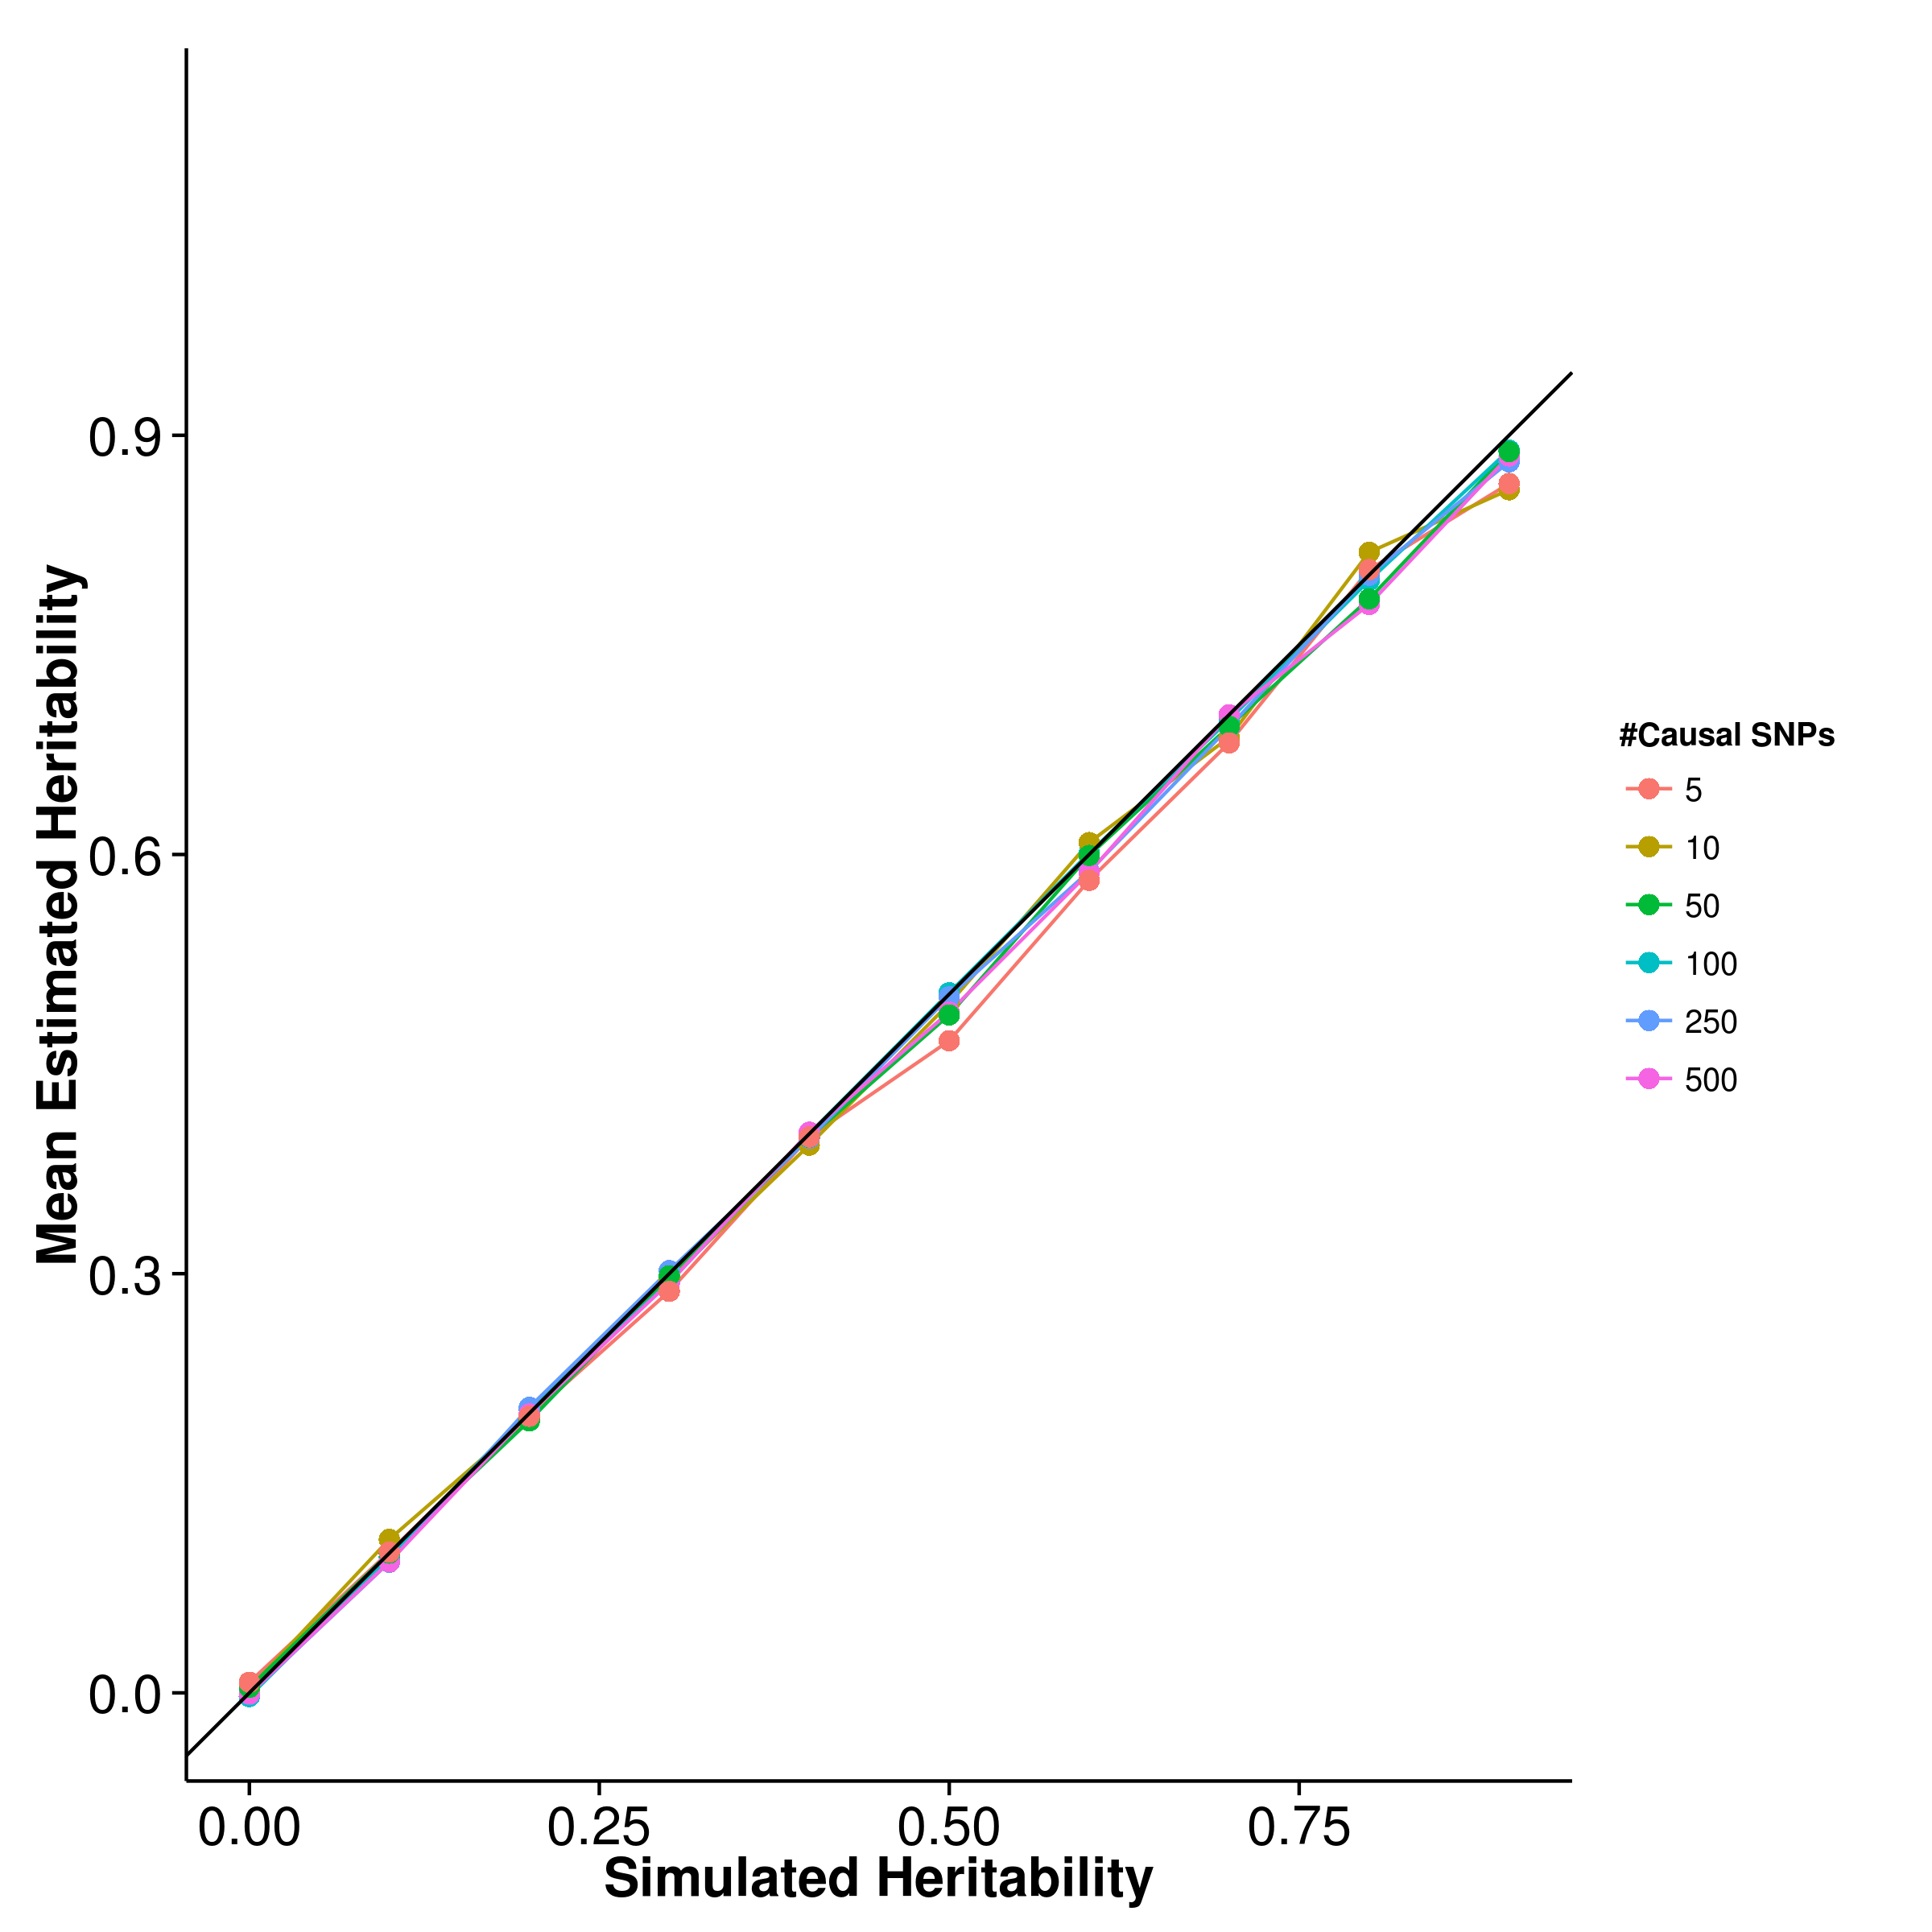
\includegraphics{figure/he_summary/random/shrek_Qt_Random_mean.png}}
				\label{fig:shrekQtRandMean}
			}
			\subfloat[GCTA]{
				\scalebox{.4}{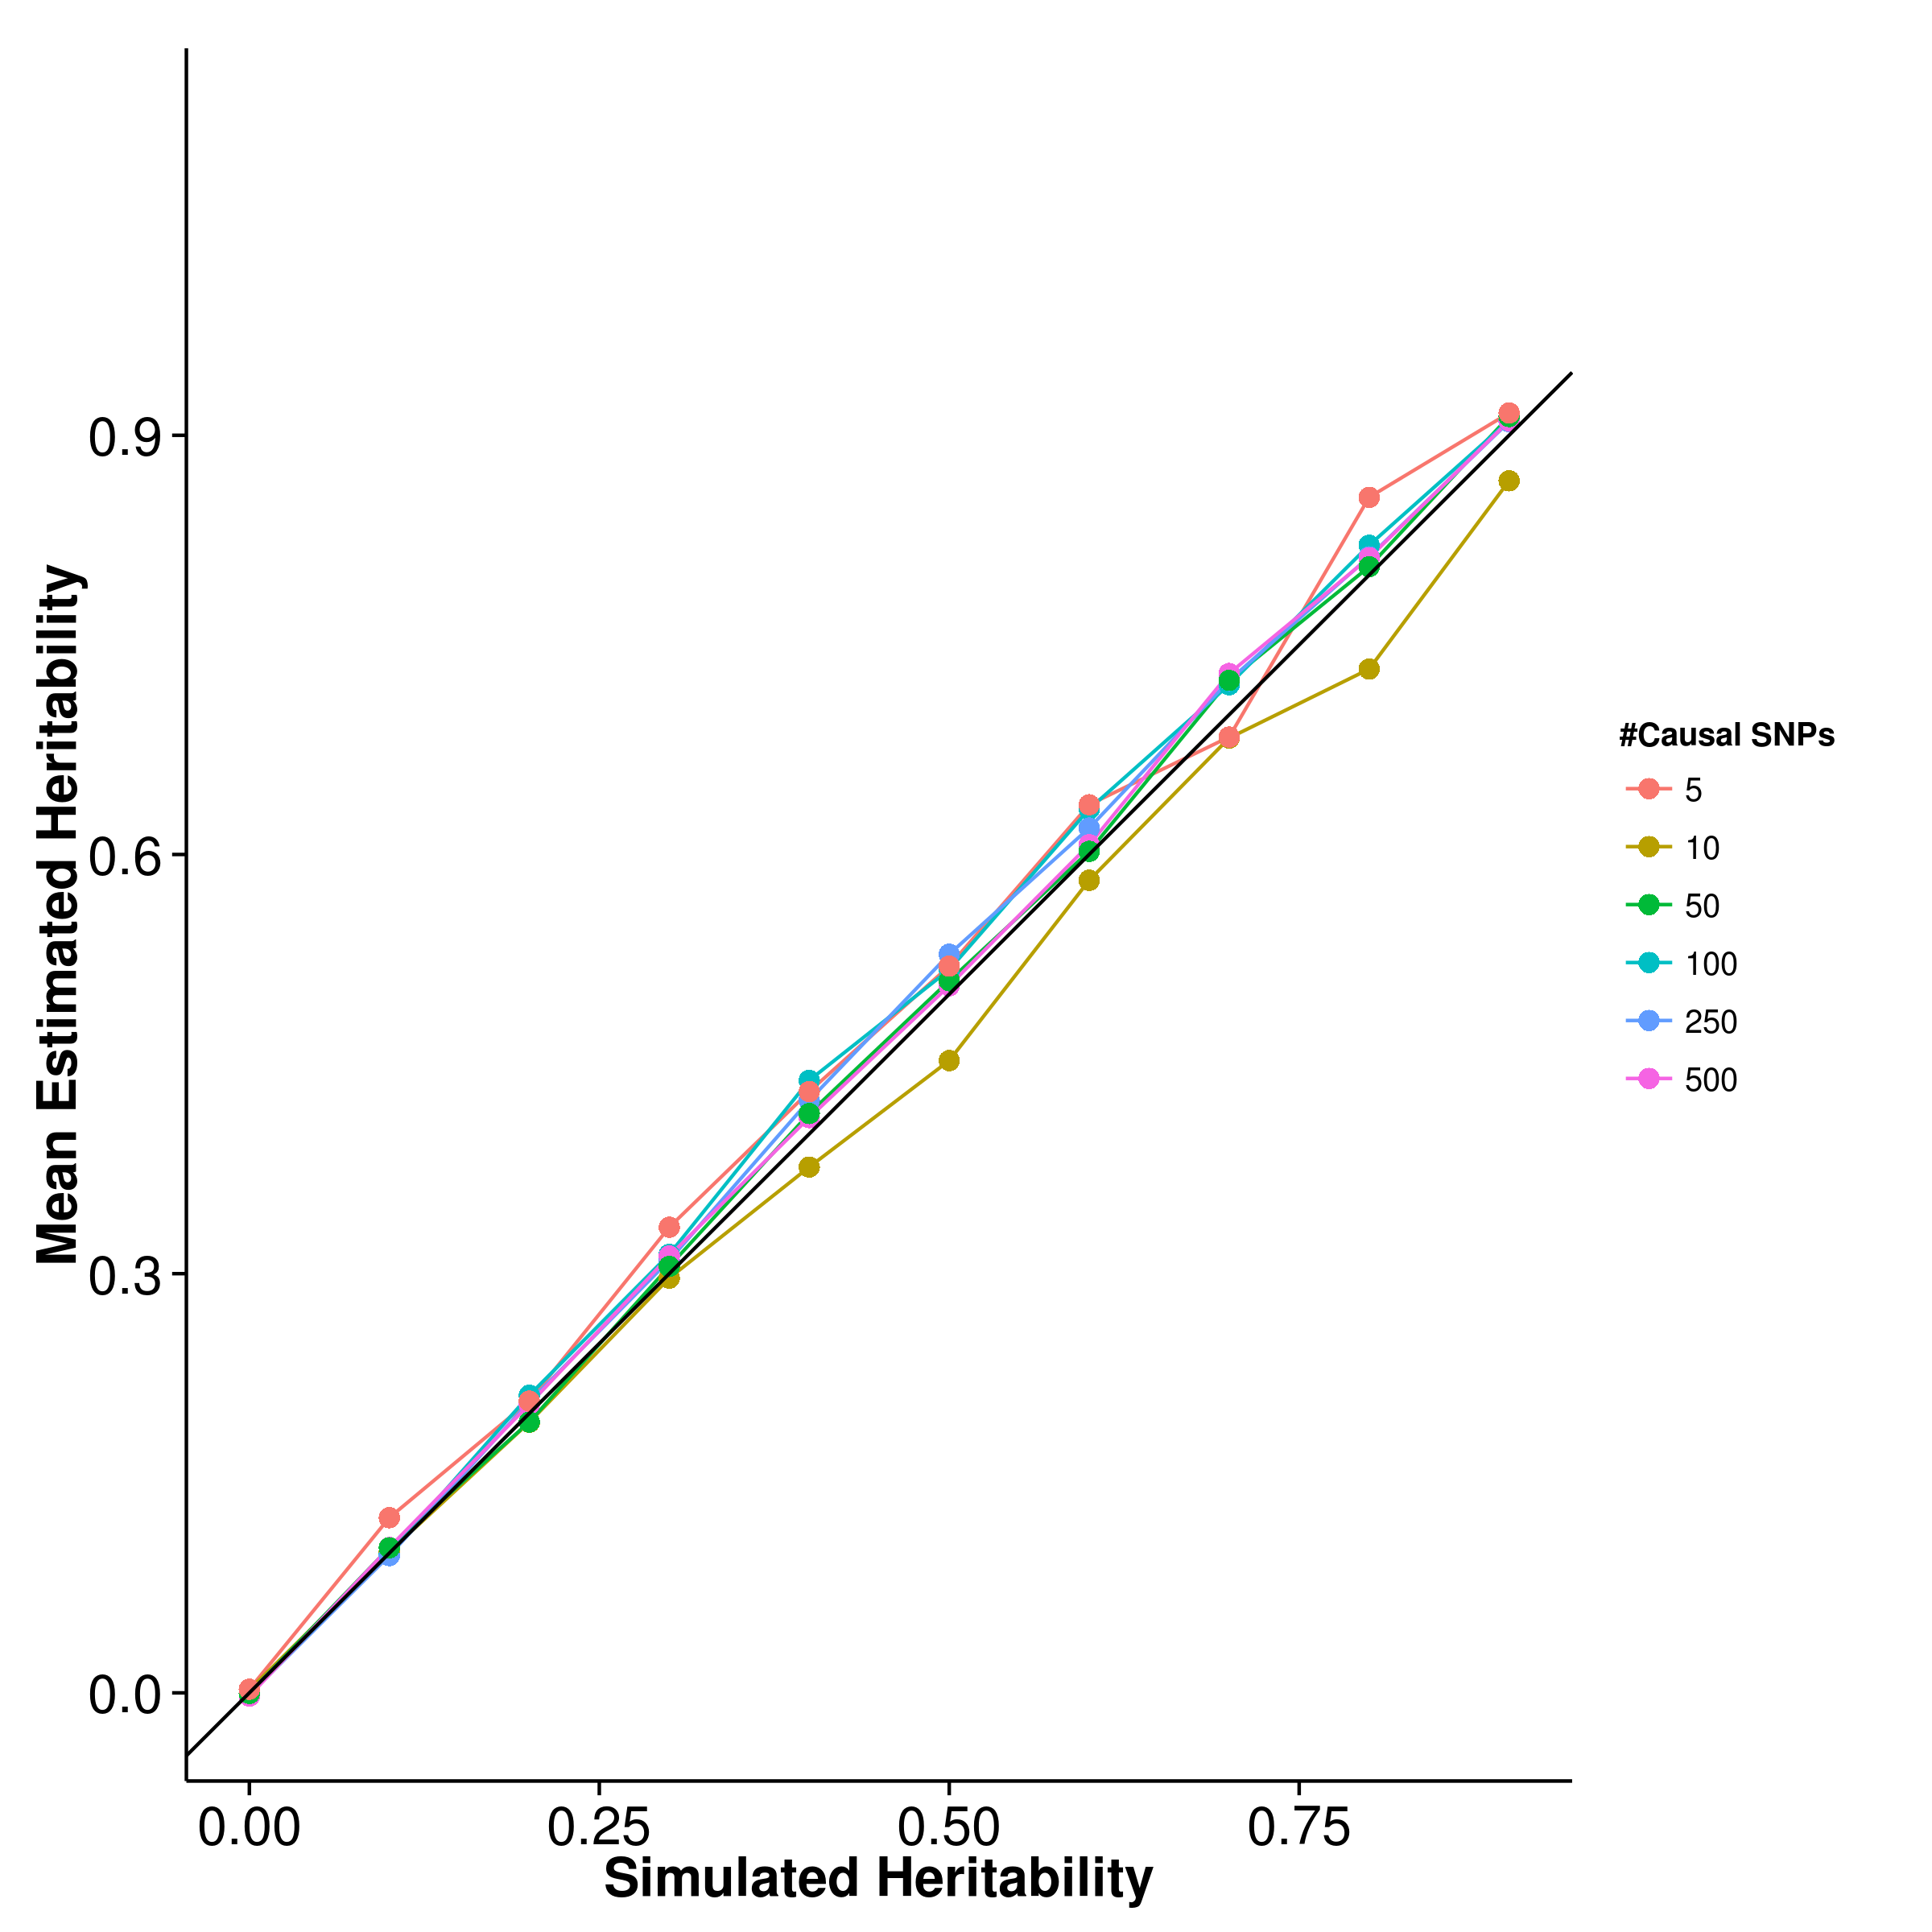
\includegraphics{figure/he_summary/random/gcta_Qt_Random_mean.png}}
				\label{fig:gctaQtRandMean}
			}\\
			\subfloat[LDSC with fix intercept]{
				\scalebox{.4}{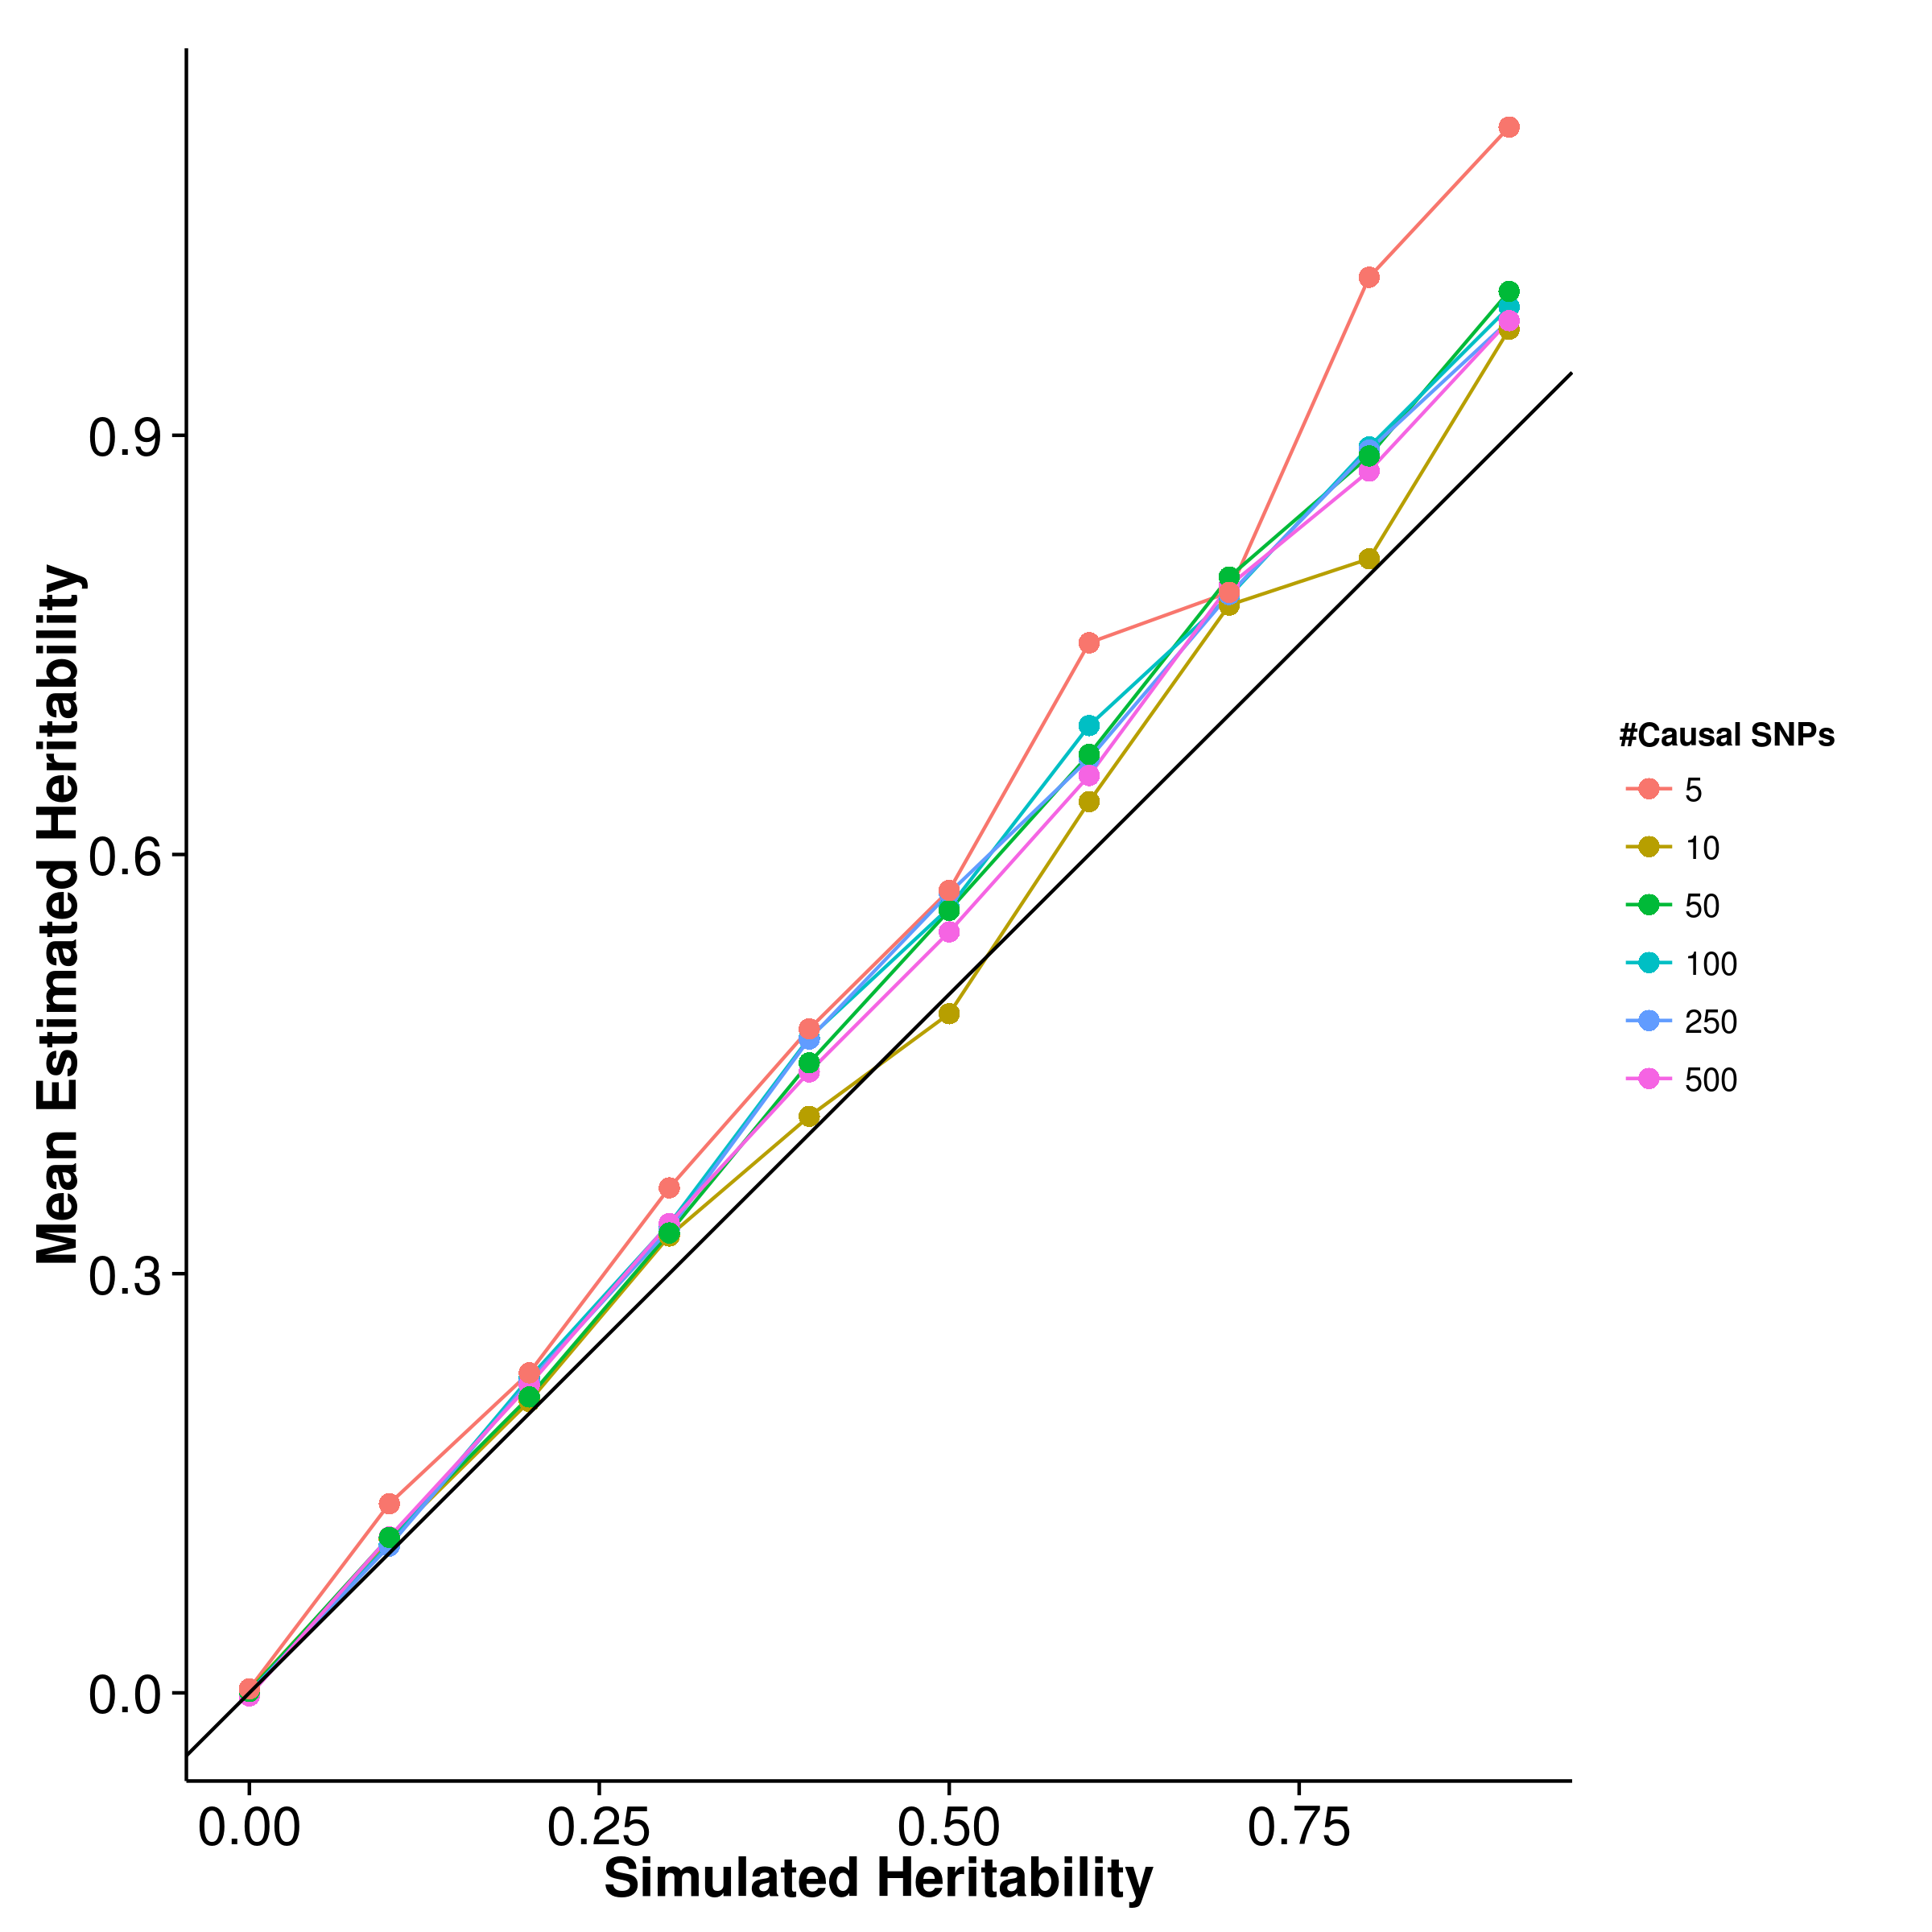
\includegraphics{figure/he_summary/random/ldsc_Qt_Random_mean.png}}
				\label{fig:ldscQtRandMean}
			}
			\subfloat[LDSC with intercept estimation]{
				
				\scalebox{.4}{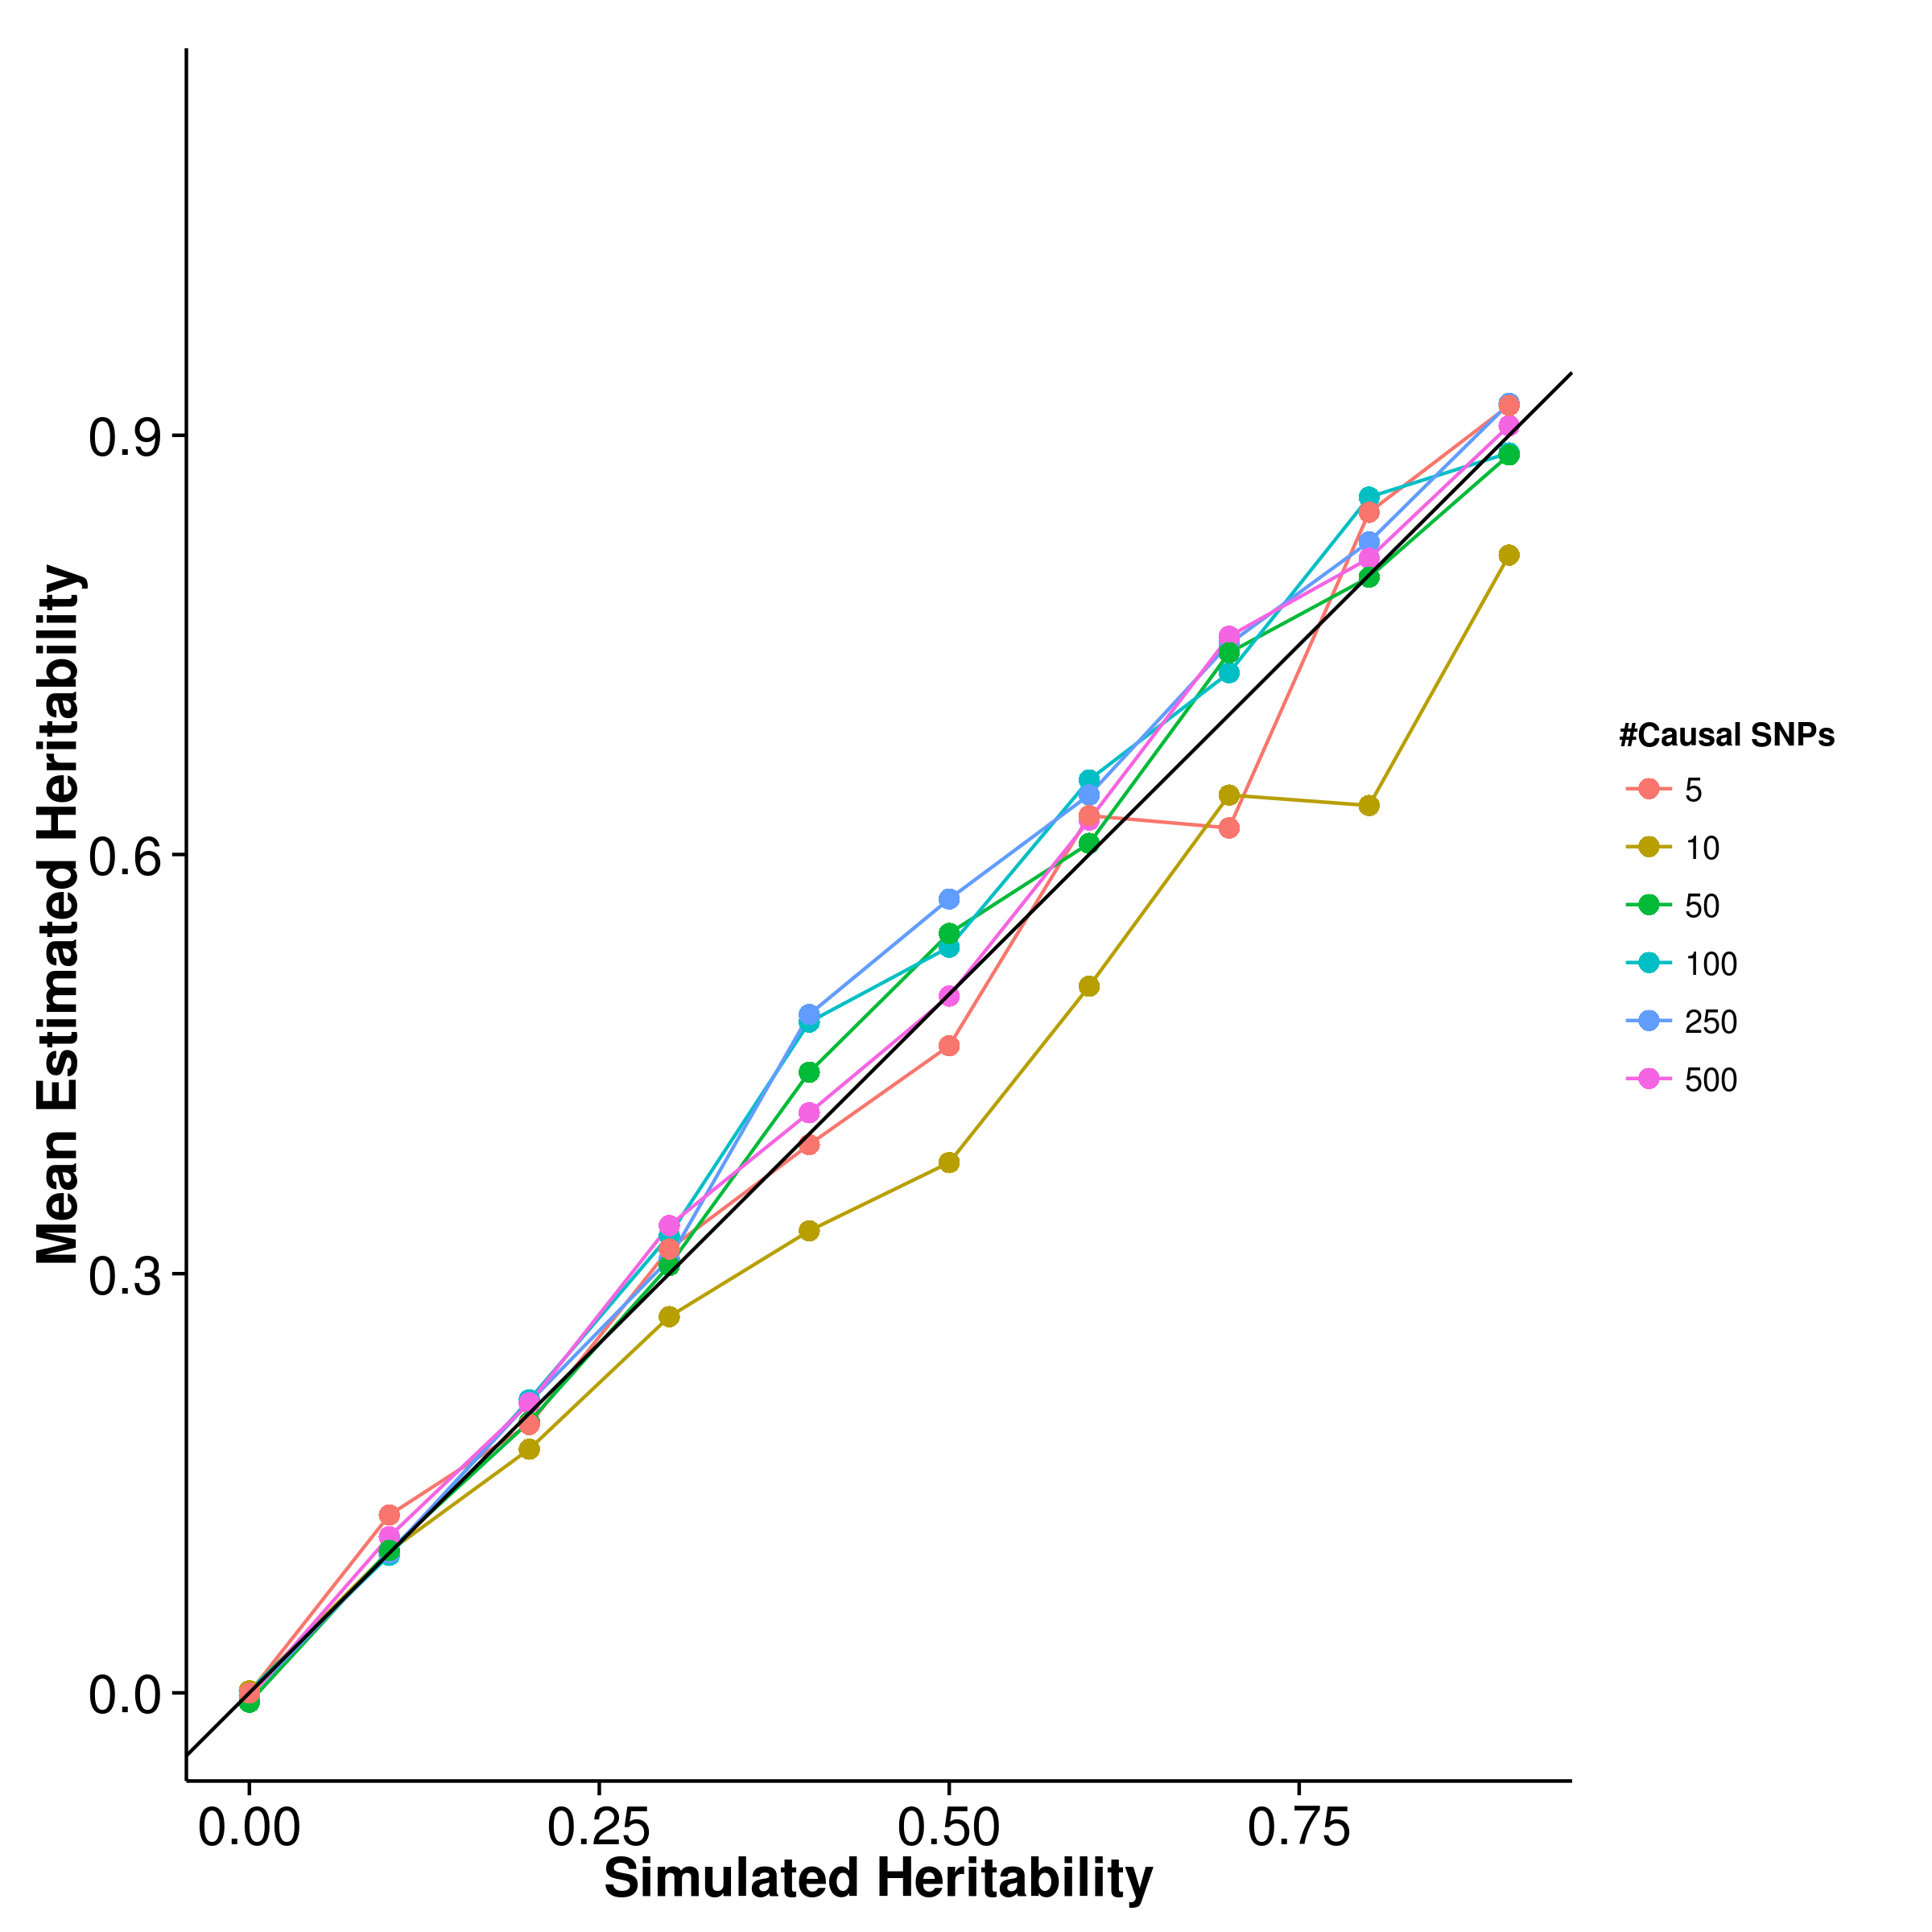
\includegraphics{figure/he_summary/random/ldscIn_Qt_Random_mean.png}}
				\label{fig:ldscInQtRandMean}
			}
			\caption[Quantitative Trait with Random Effect Size Simulation Result(Mean)]
			{Mean of results from quantitative trait simulation with random effect size simulation.
				The result was very much similar to the condition where a equal effect size was simulated.
				Again, \gls{shrek} has the most accurate mean estimate when compared to other tools, with \gls{ldsc} slightly inflated.} 
			\label{fig:QtRandMean}
		\end{figure}
		
		\begin{figure}
			\centering
			\subfloat[SHREK]{
				\scalebox{.4}{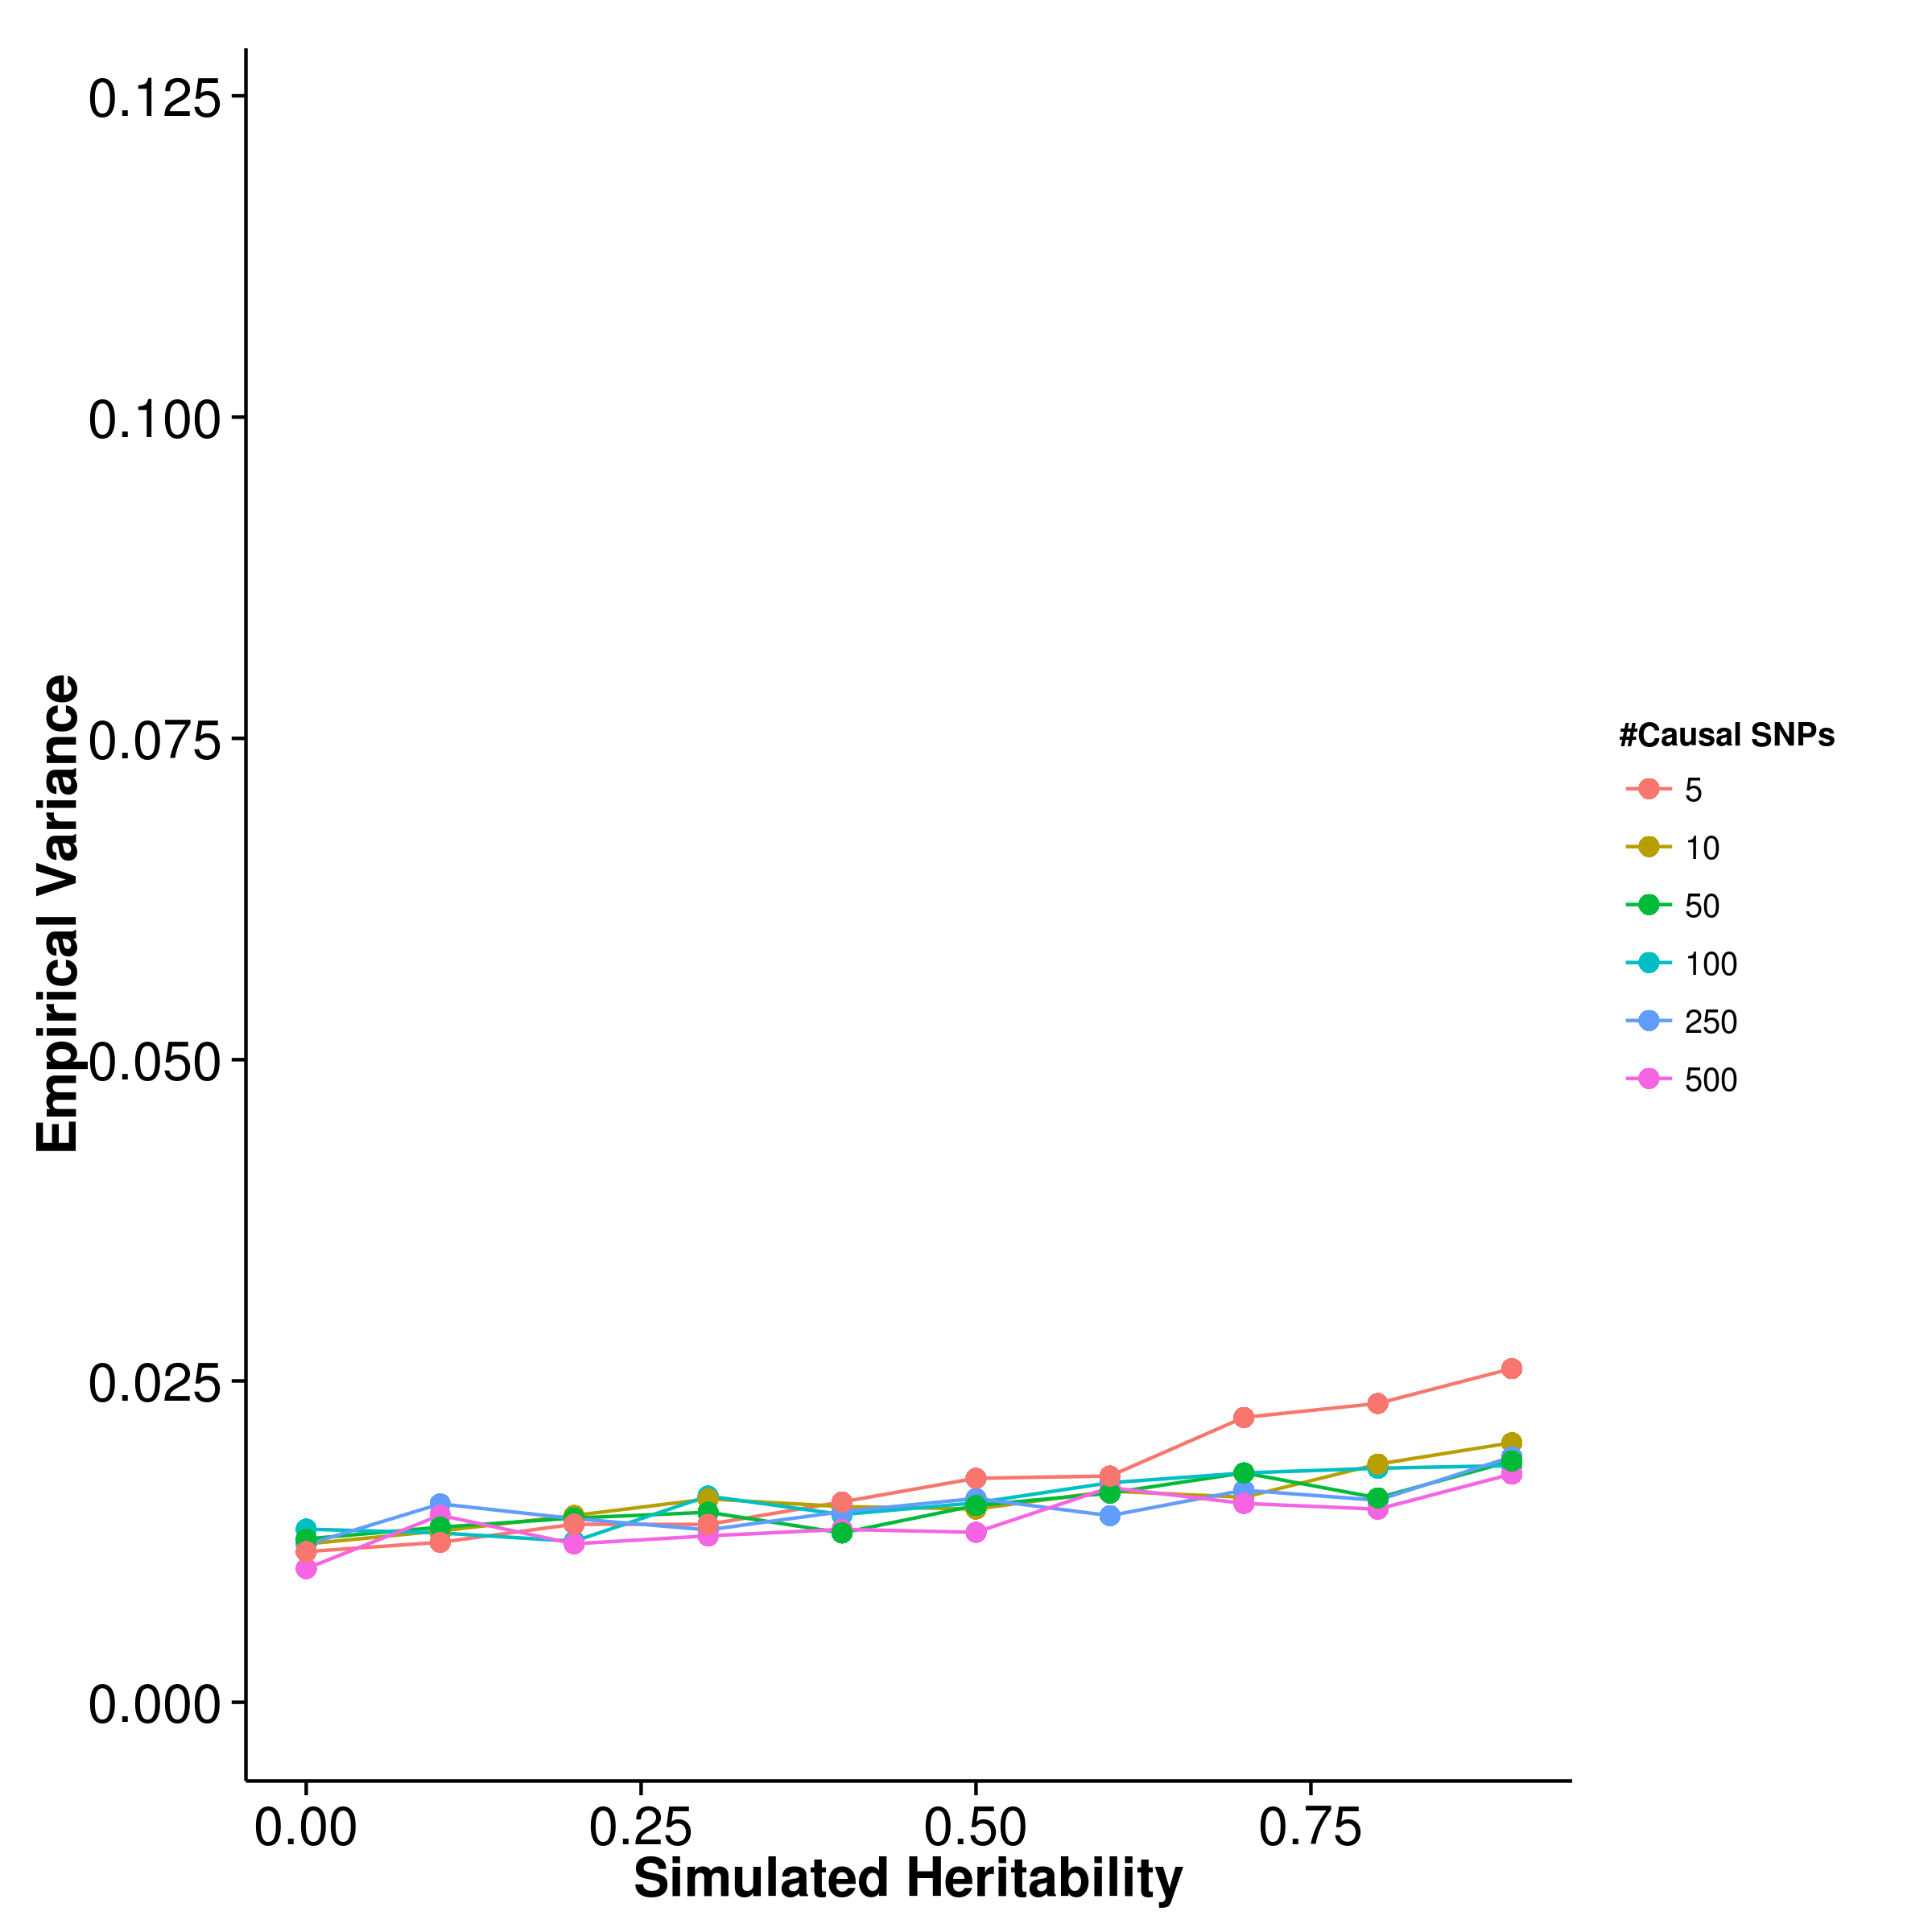
\includegraphics{figure/he_summary/random/shrek_Qt_Random_sd.png}}
				\label{fig:shrekQtRandVar}
			}
			\subfloat[GCTA]{
				\scalebox{.4}{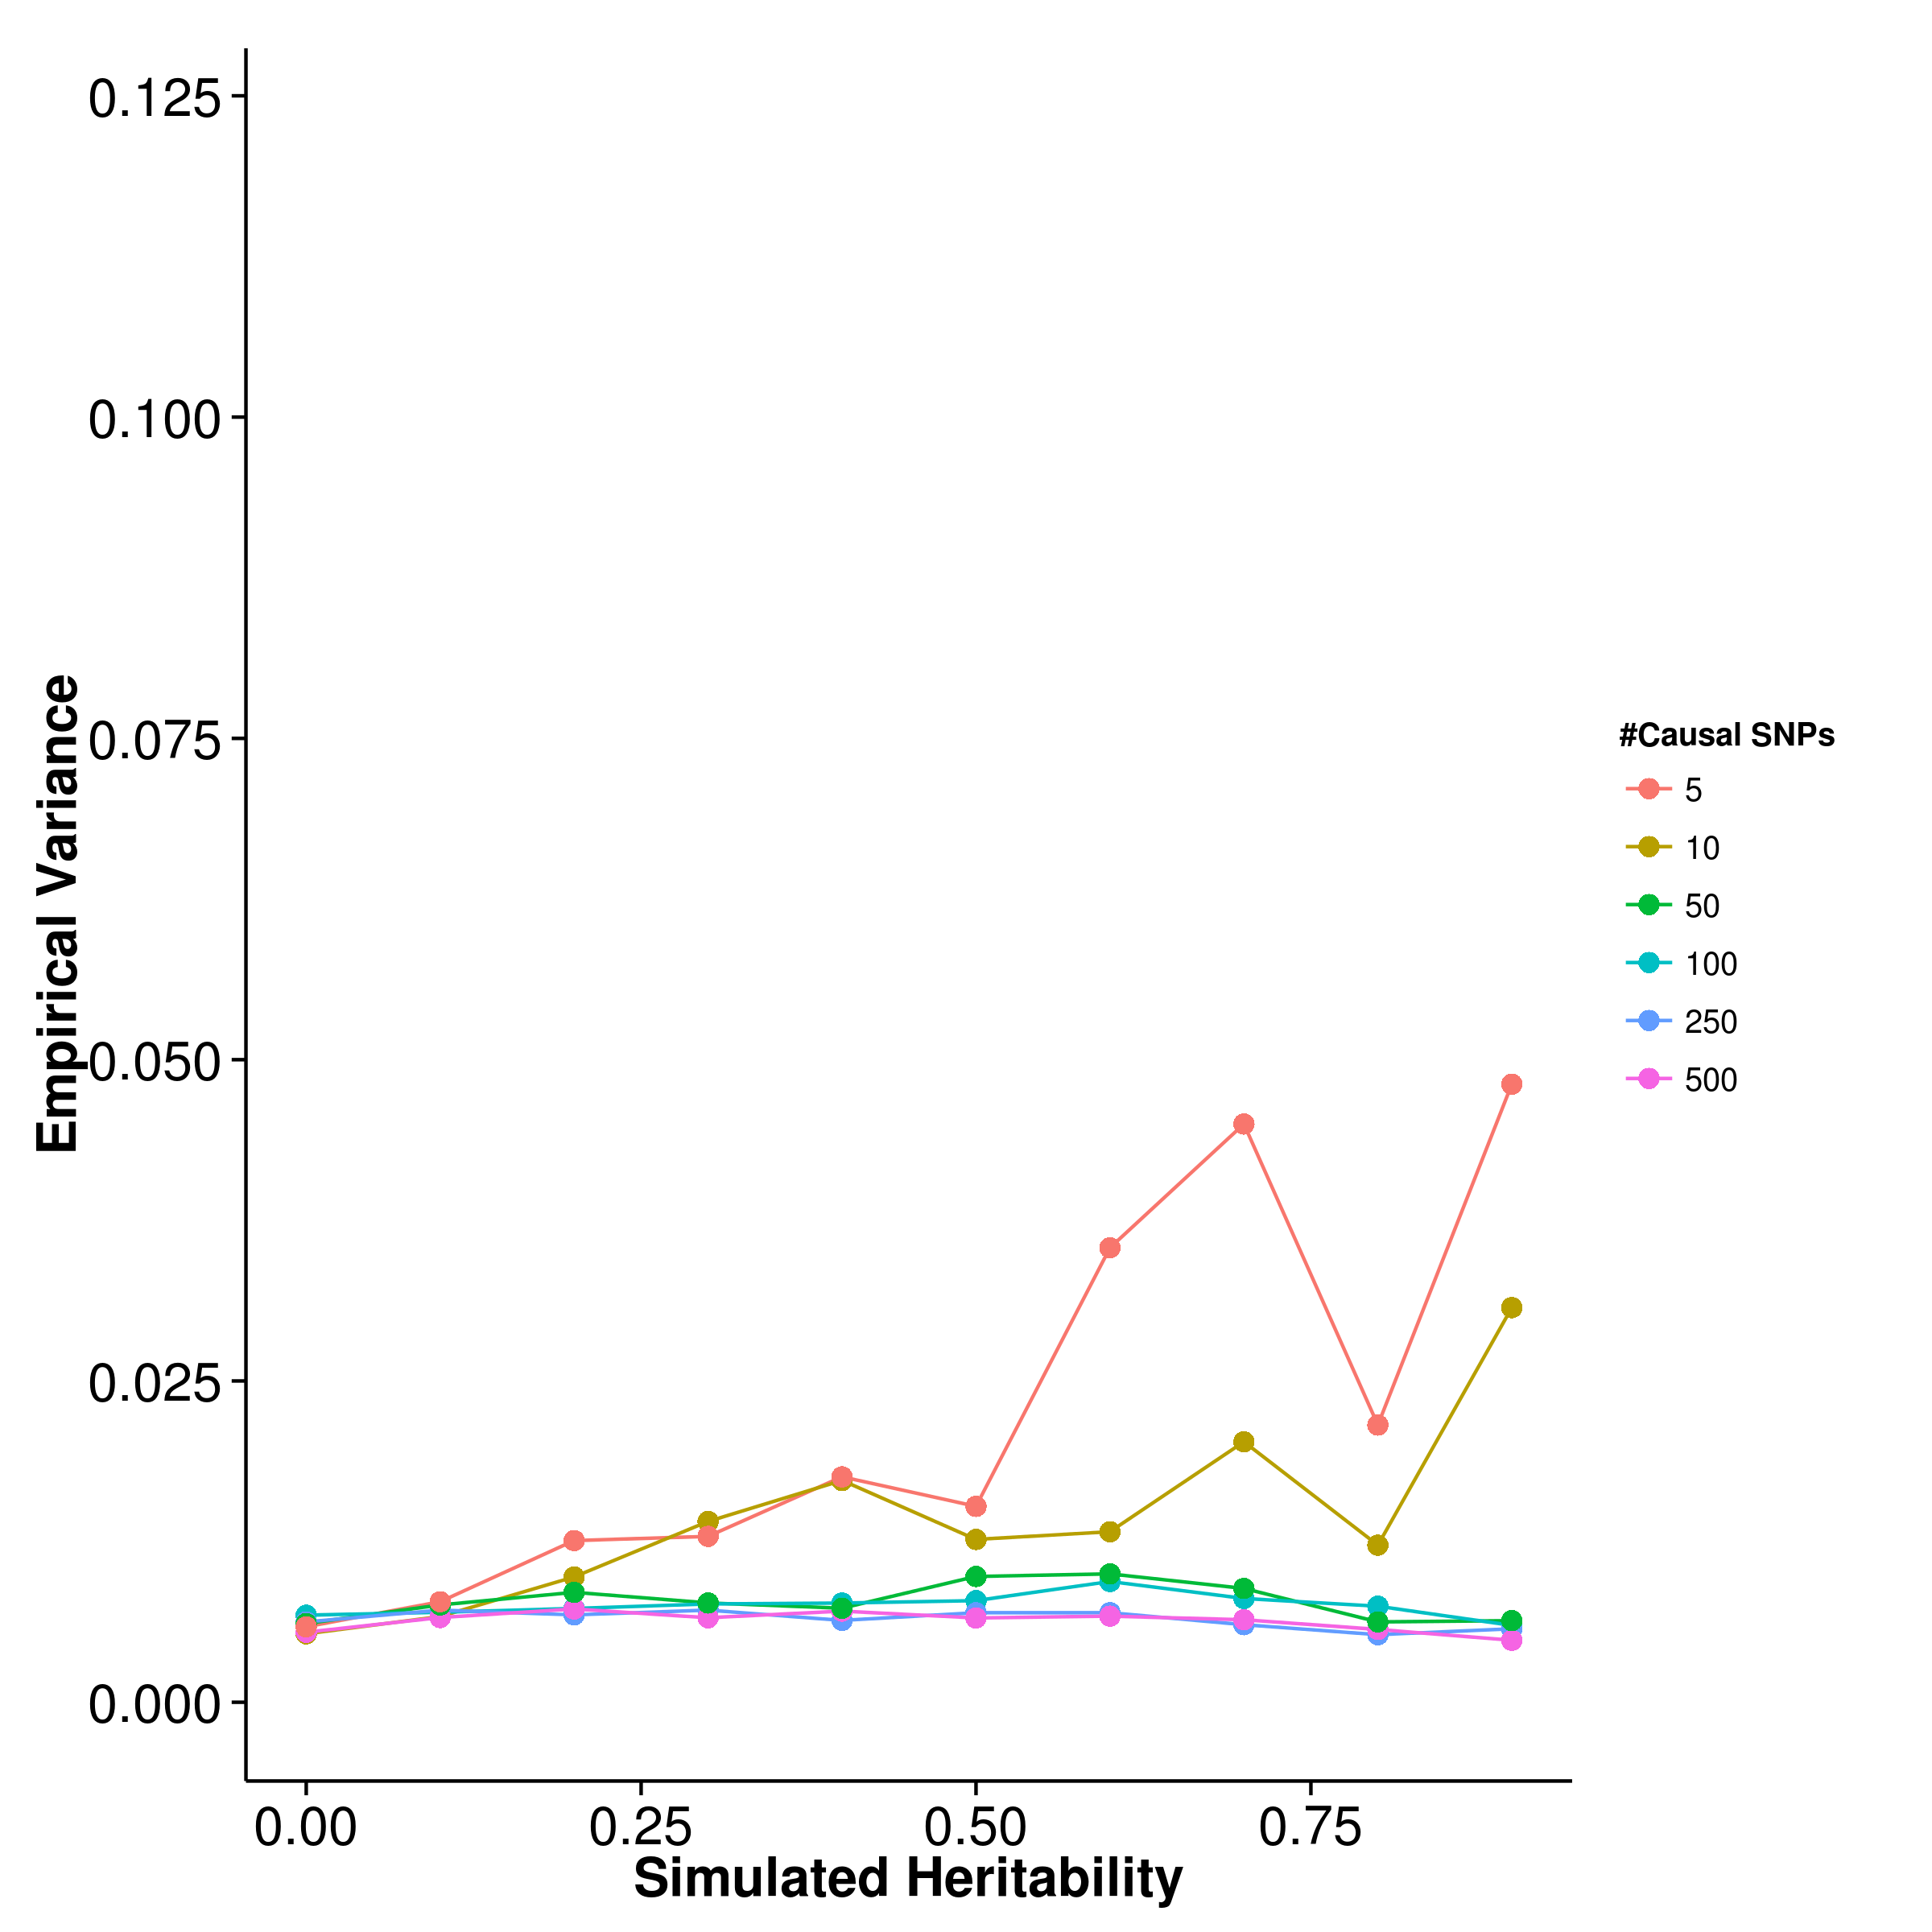
\includegraphics{figure/he_summary/random/gcta_Qt_Random_sd.png}}
				\label{fig:gctaQtRandVar}
			}\\
			\subfloat[LDSC with fix intercept]{
				\scalebox{.4}{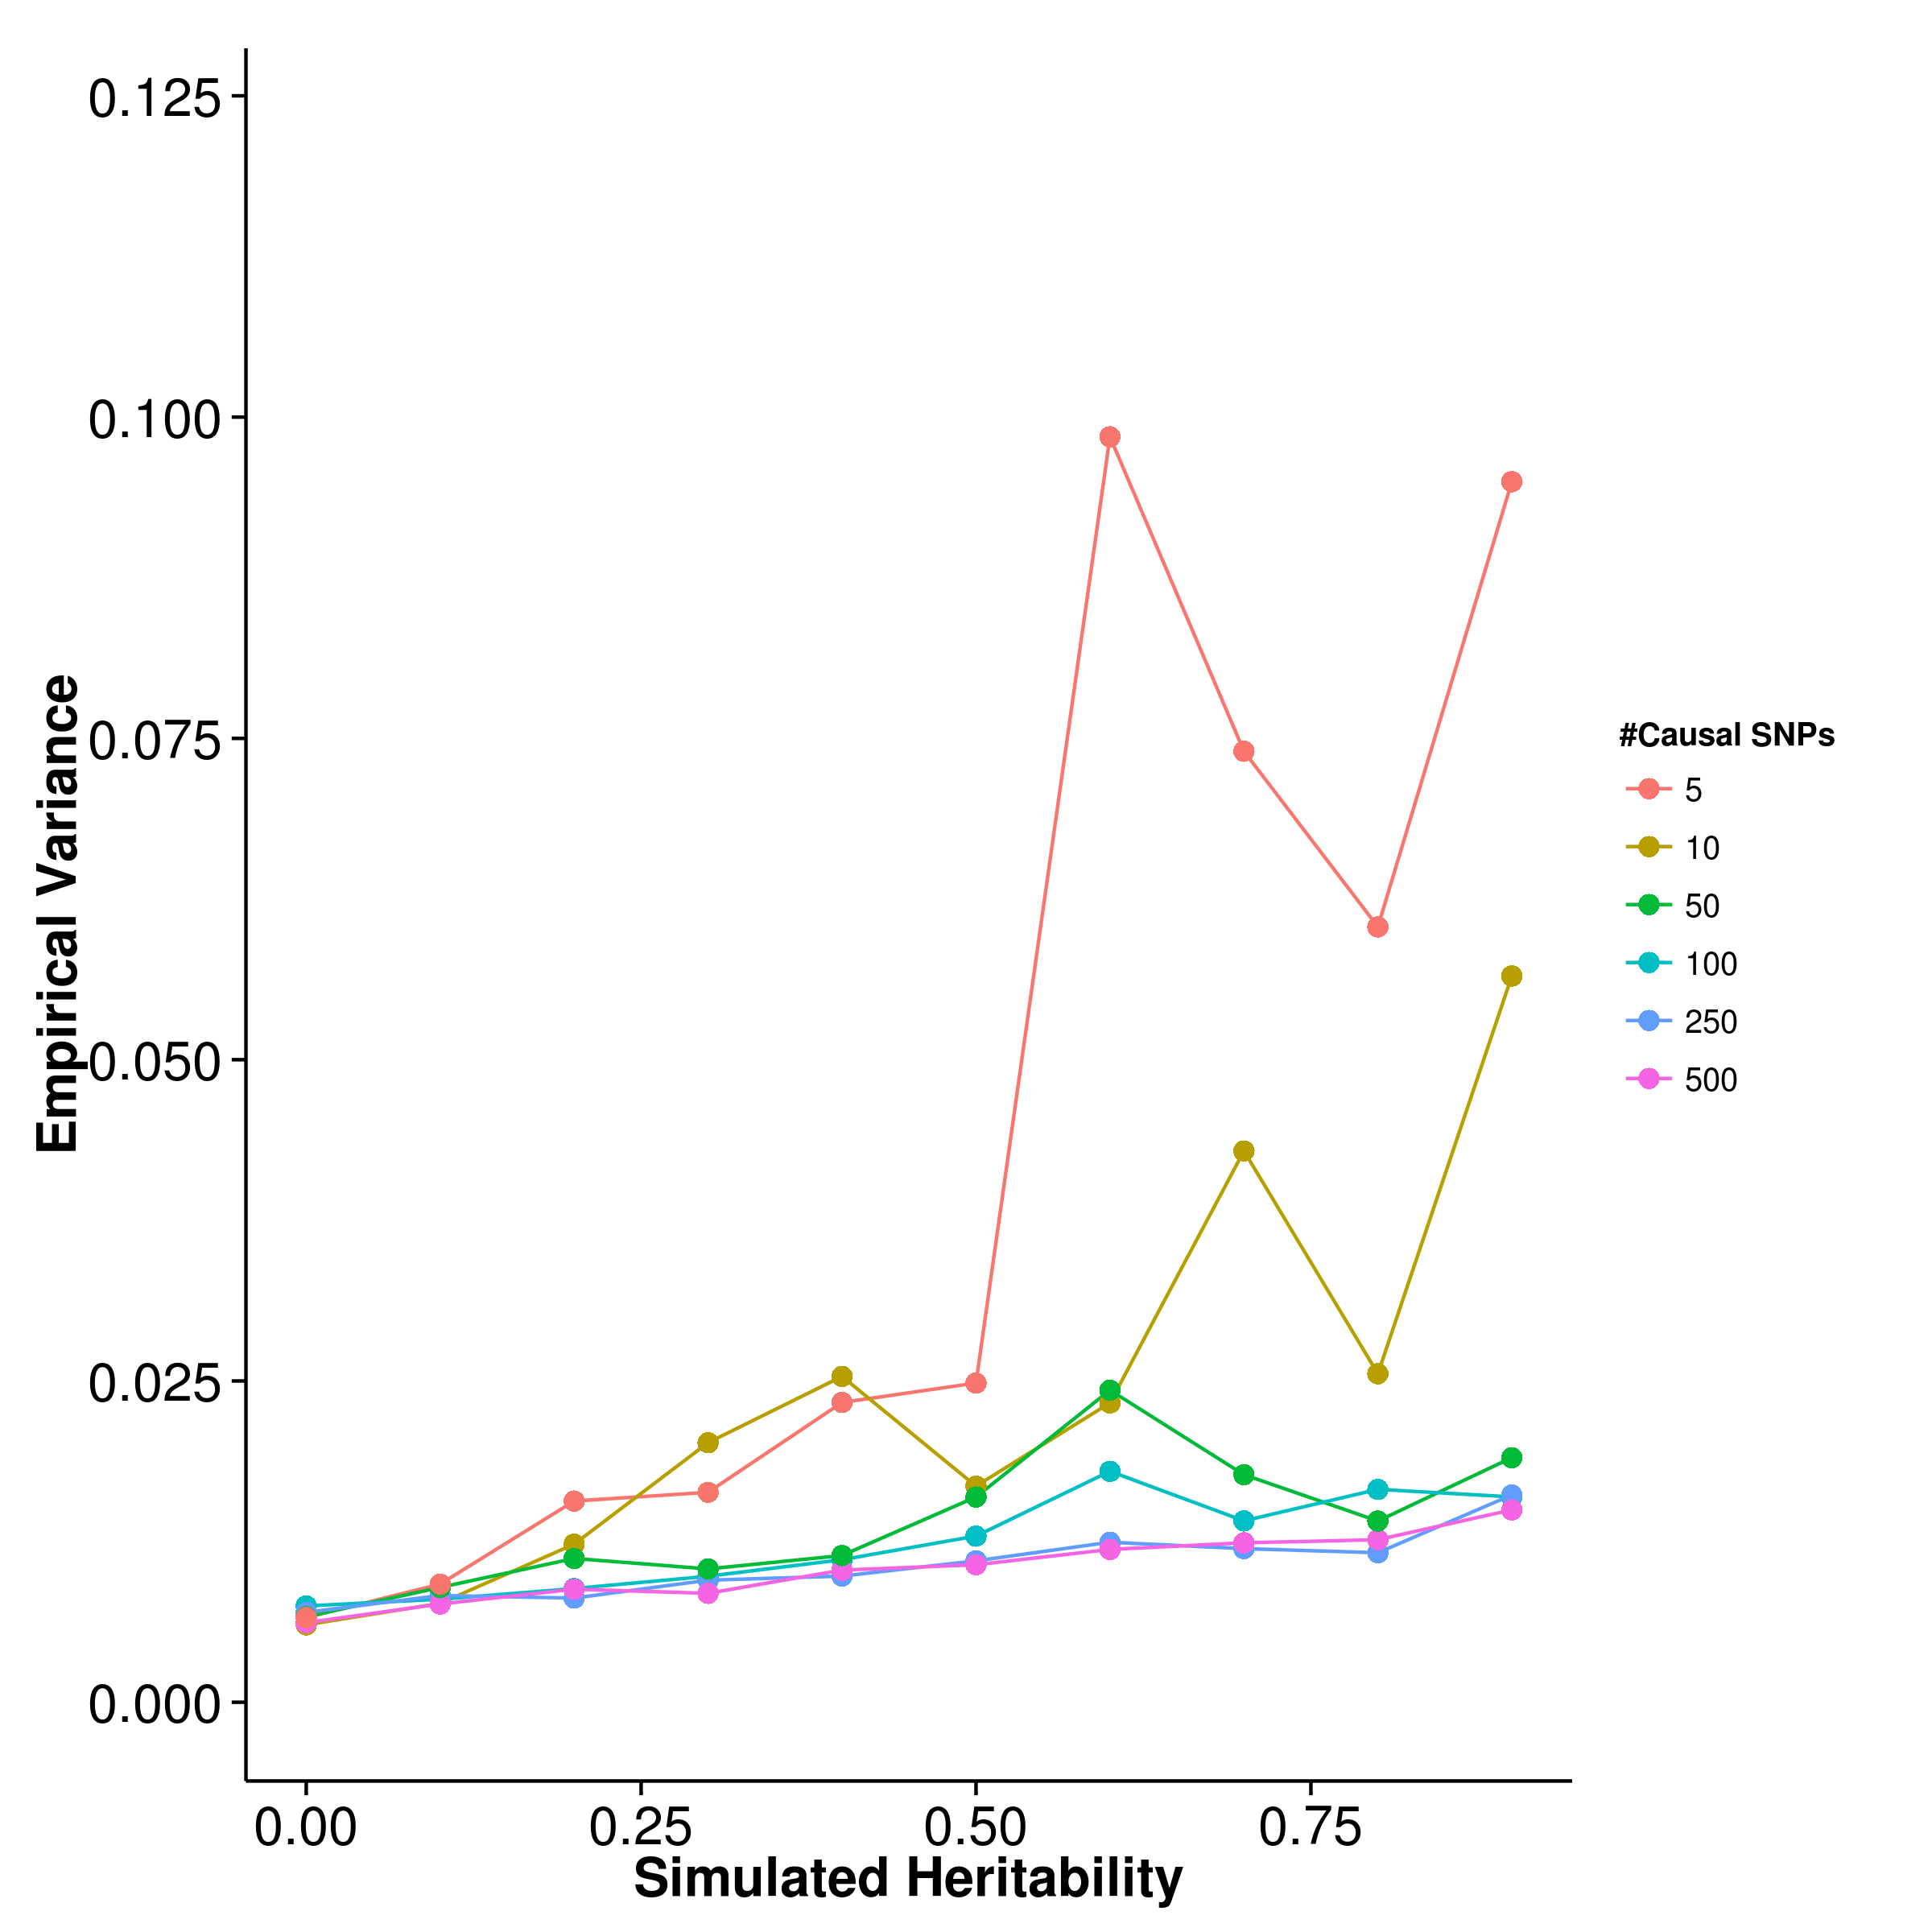
\includegraphics{figure/he_summary/random/ldsc_Qt_Random_sd.png}}
				\label{fig:ldscQtRandVar}
			}
			\subfloat[LDSC with intercept estimation]{
				
				\scalebox{.4}{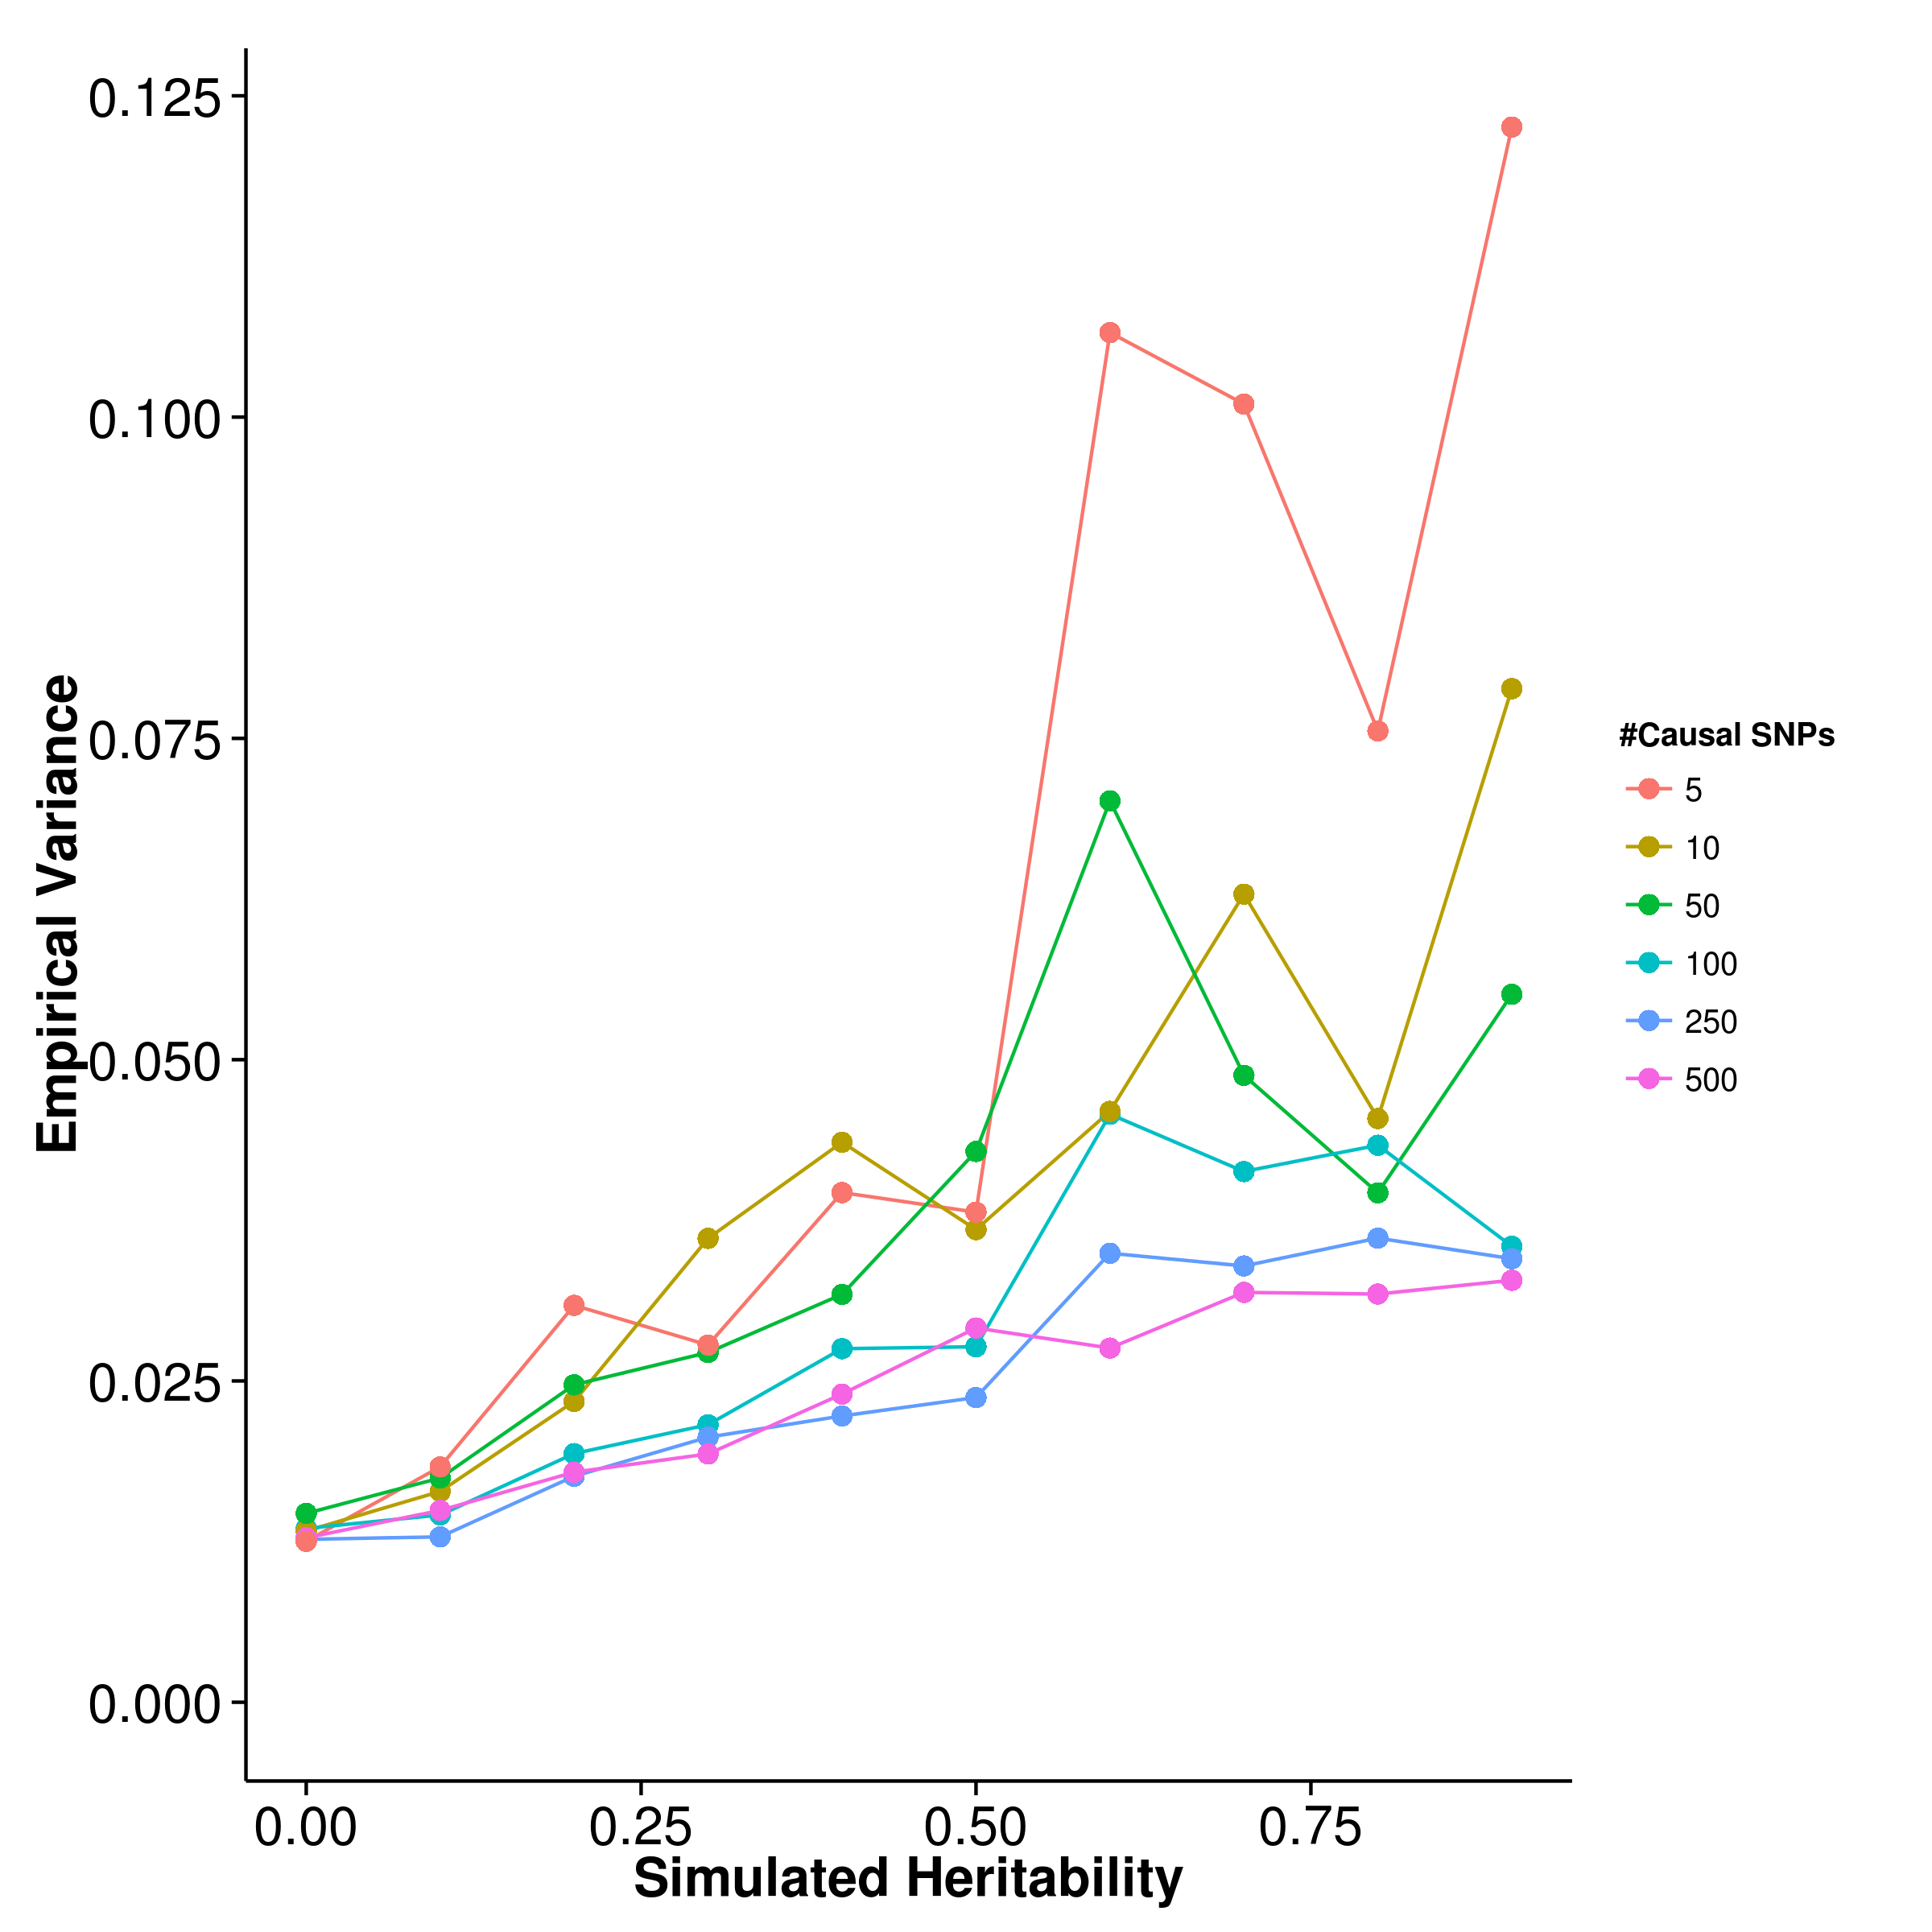
\includegraphics{figure/he_summary/random/ldscIn_Qt_Random_sd.png}}
				\label{fig:ldscInQtRandVar}
			}
			\caption[Quantitative Trait with Random Effect Size Simulation Result(Variance)]
			{Variance of results from quantitative trait simulation with random effect size simulation.
				Again, the variance of the estimate were almost the same as in simulation of equal effect size where \gls{gcta} has the smallest variance, follow by \gls{ldsc}. 
				However, it was observed when the number of causal \glspl{SNP} decreases, the variance of the estimation increases for all programme, with variance of the \gls{shrek} estimate being the least sensitive to change in heritability.
			} 
			\label{fig:QtRandVar}
		\end{figure}
		
		\begin{figure}
			\centering
			\subfloat[SHREK]{
				\scalebox{.4}{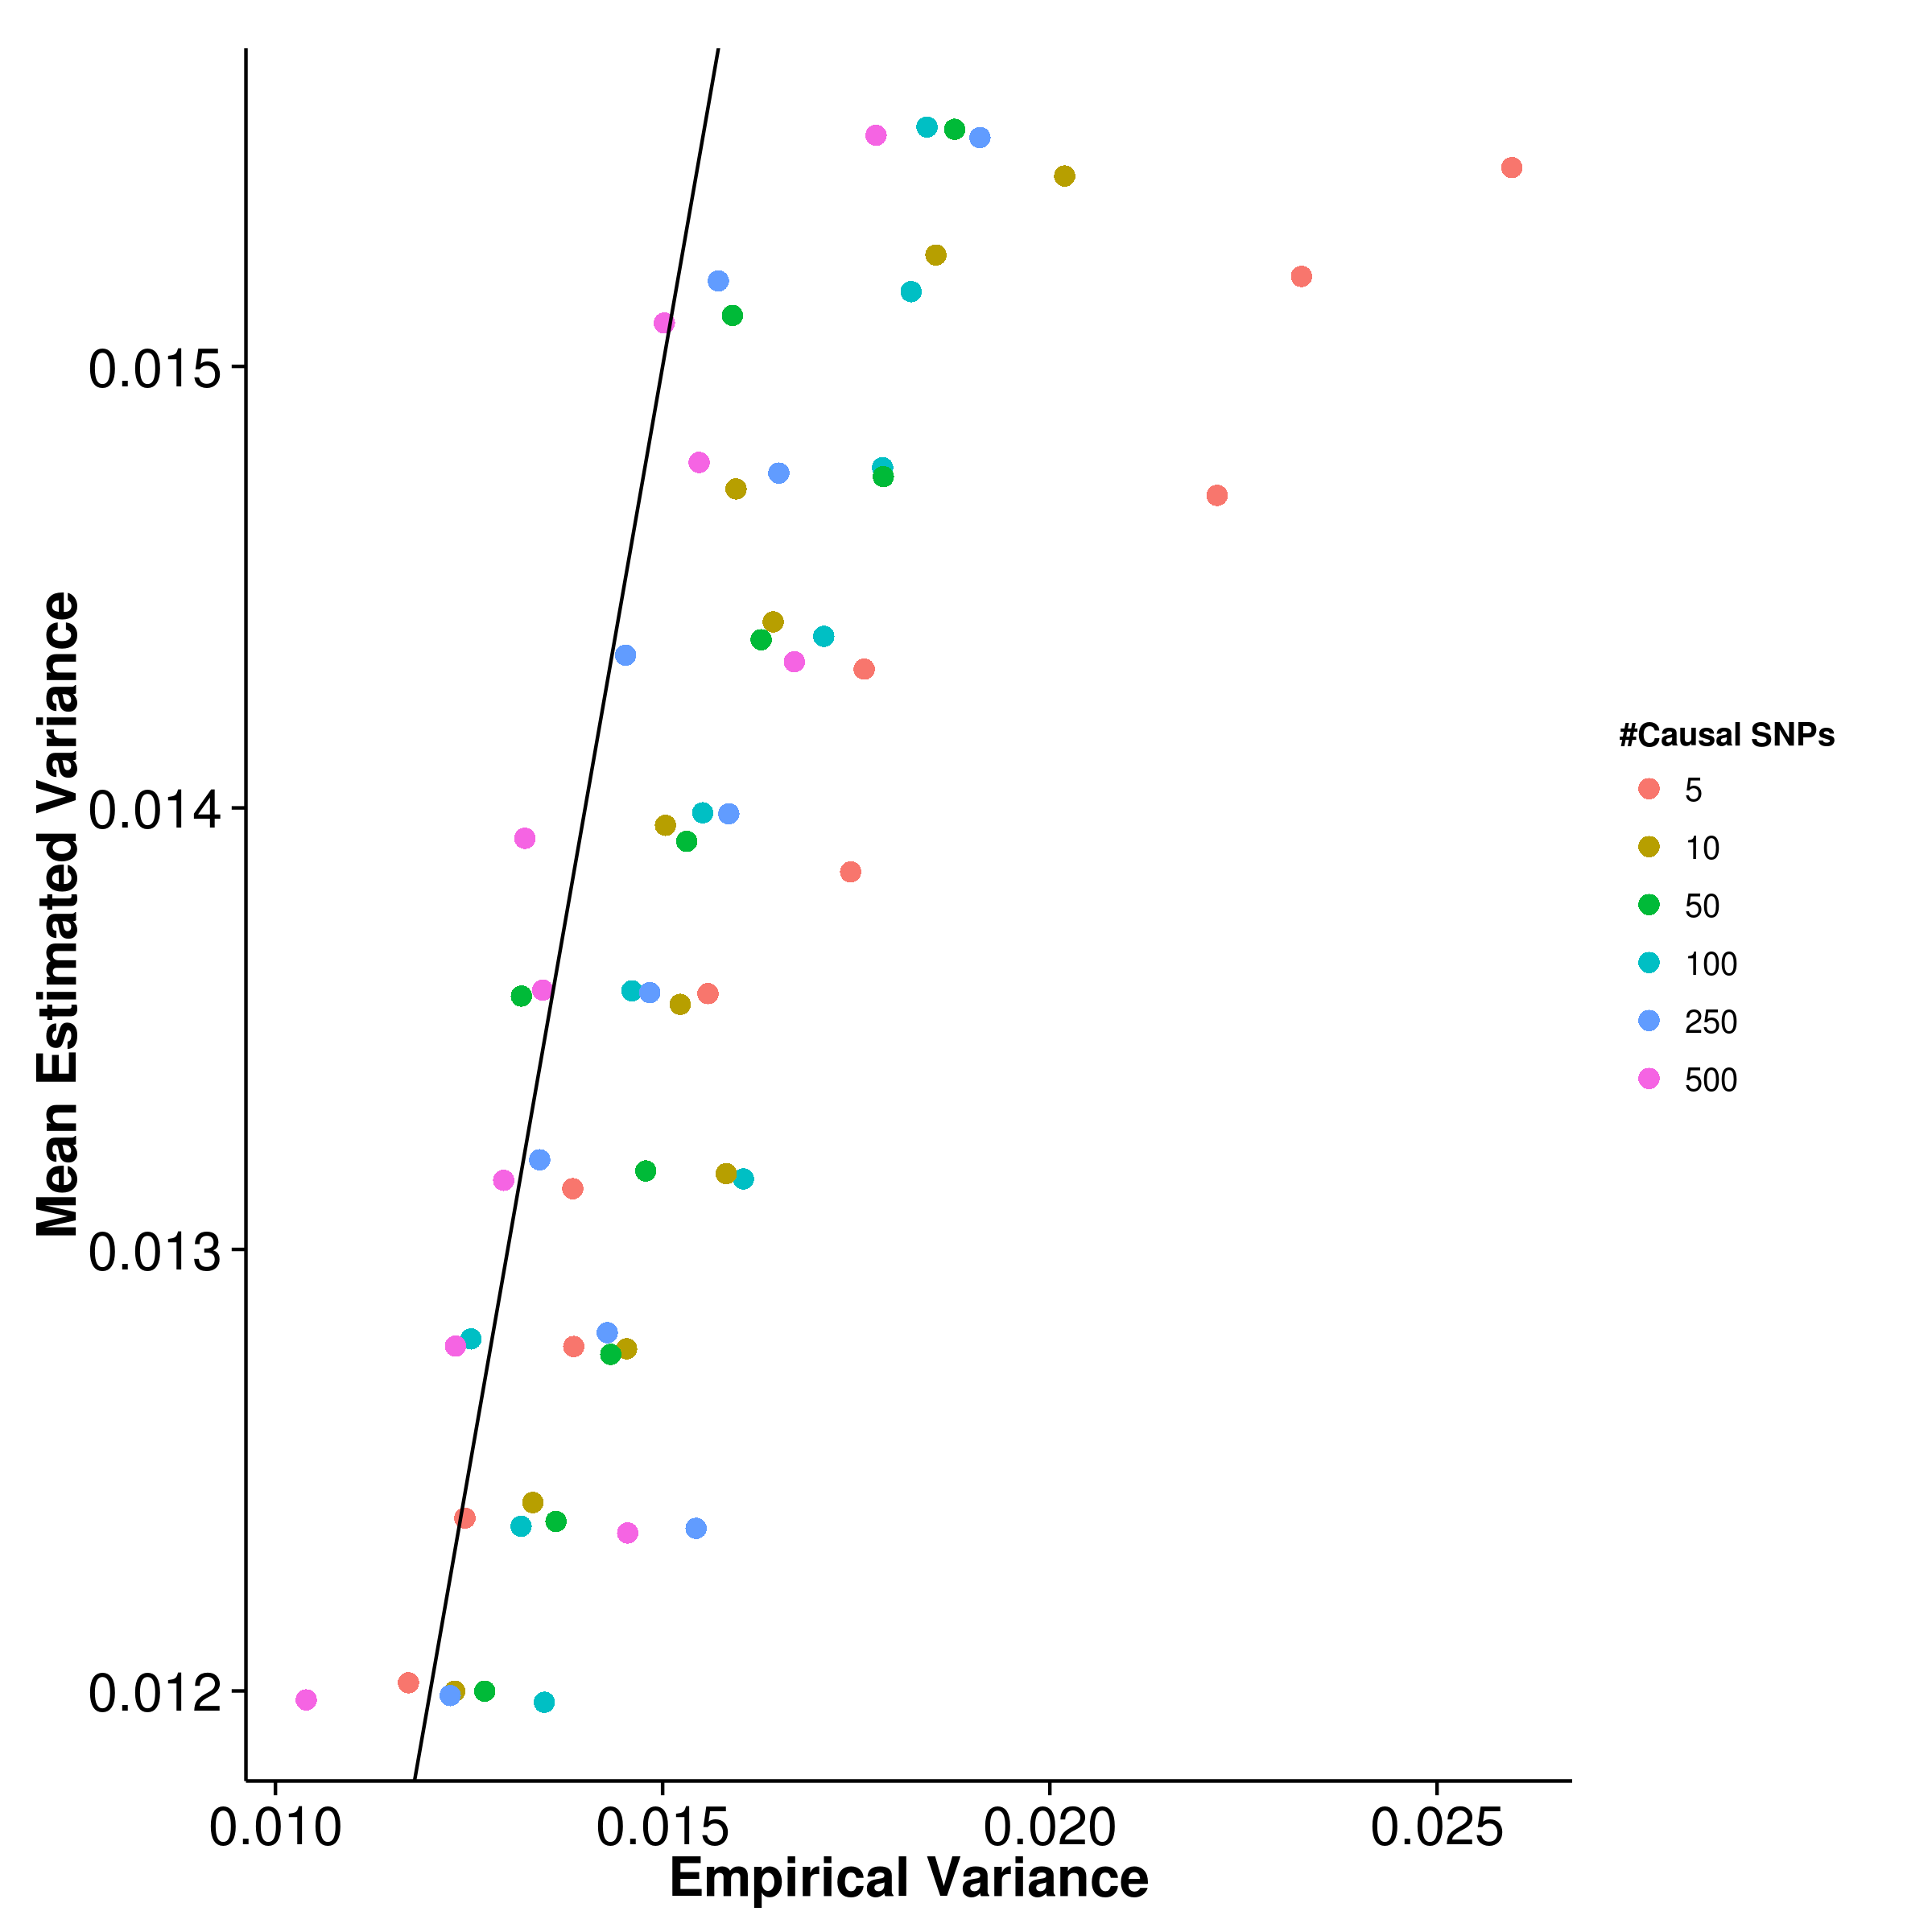
\includegraphics{figure/he_summary/random/shrek_Qt_Random_sdCom.png}}
				\label{fig:shrekQtRandVarCom}
			}
			\subfloat[GCTA]{
				\scalebox{.4}{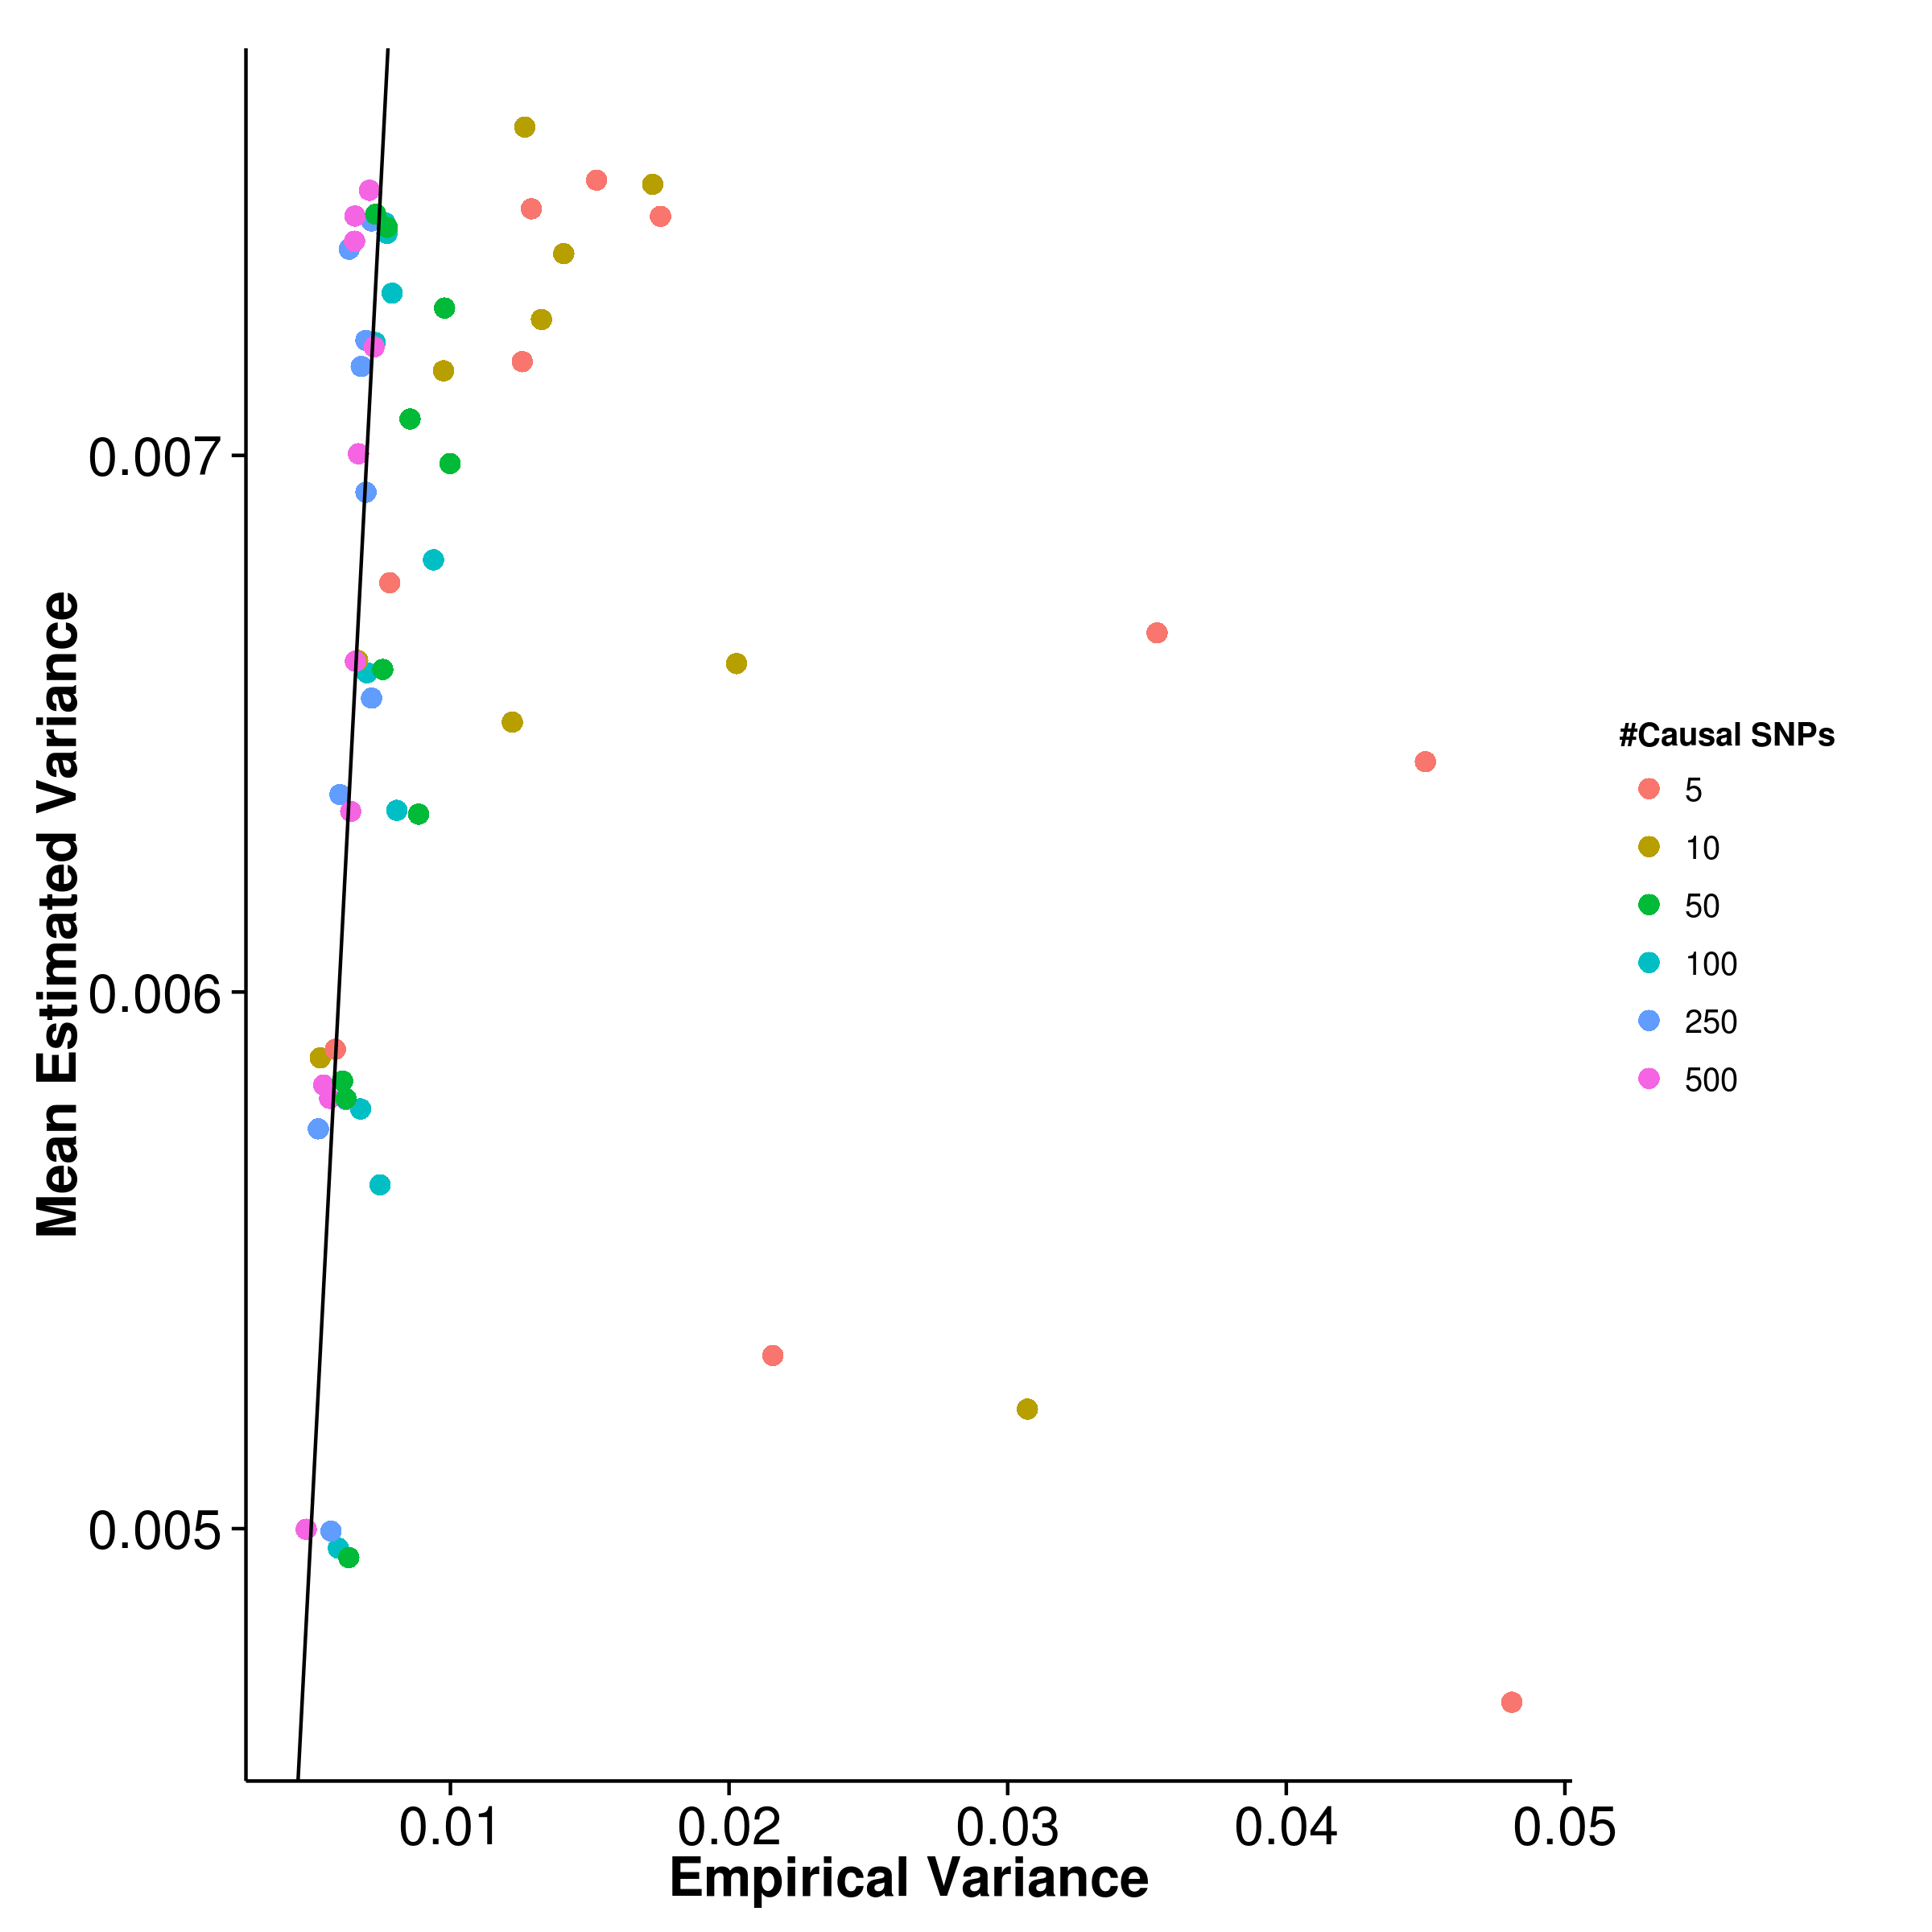
\includegraphics{figure/he_summary/random/gcta_Qt_Random_sdCom.png}}
				\label{fig:gctaQtRandVarCom}
			}\\
			\subfloat[LDSC with fix intercept]{
				\scalebox{.4}{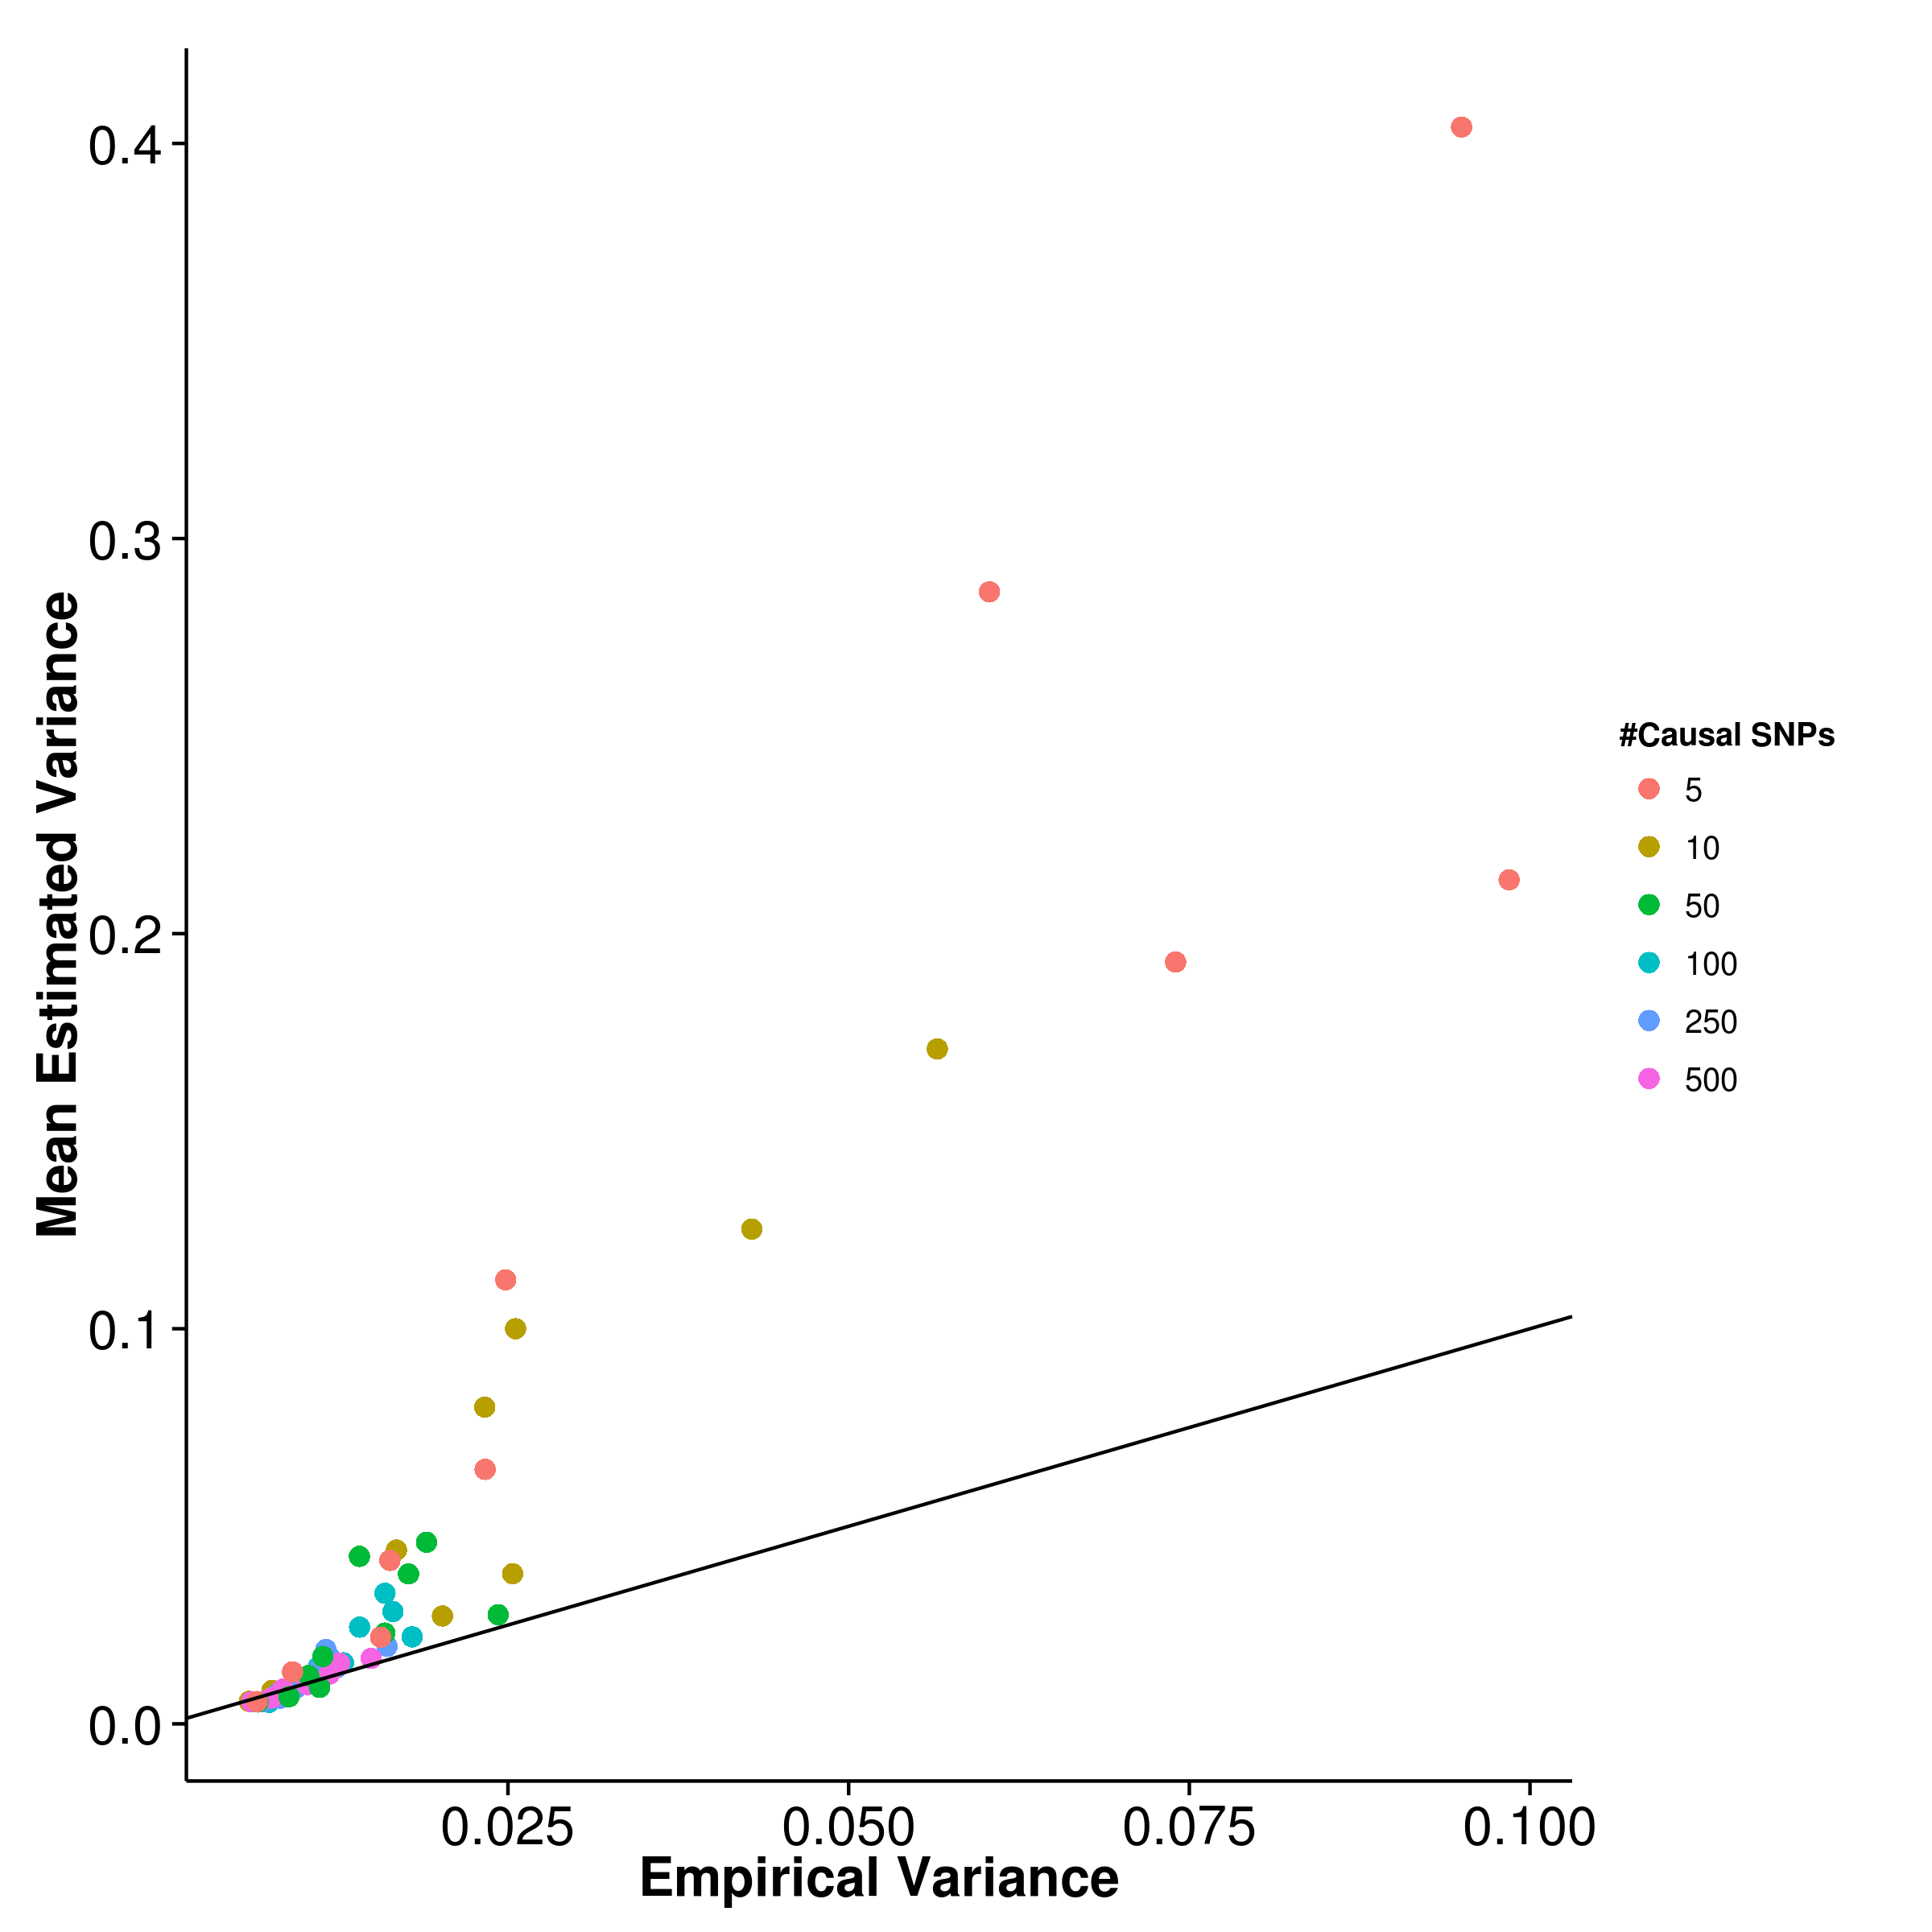
\includegraphics{figure/he_summary/random/ldsc_Qt_Random_sdCom.png}}
				\label{fig:ldscQtRandVarCom}
			}
			\subfloat[LDSC with intercept estimation]{
				
				\scalebox{.4}{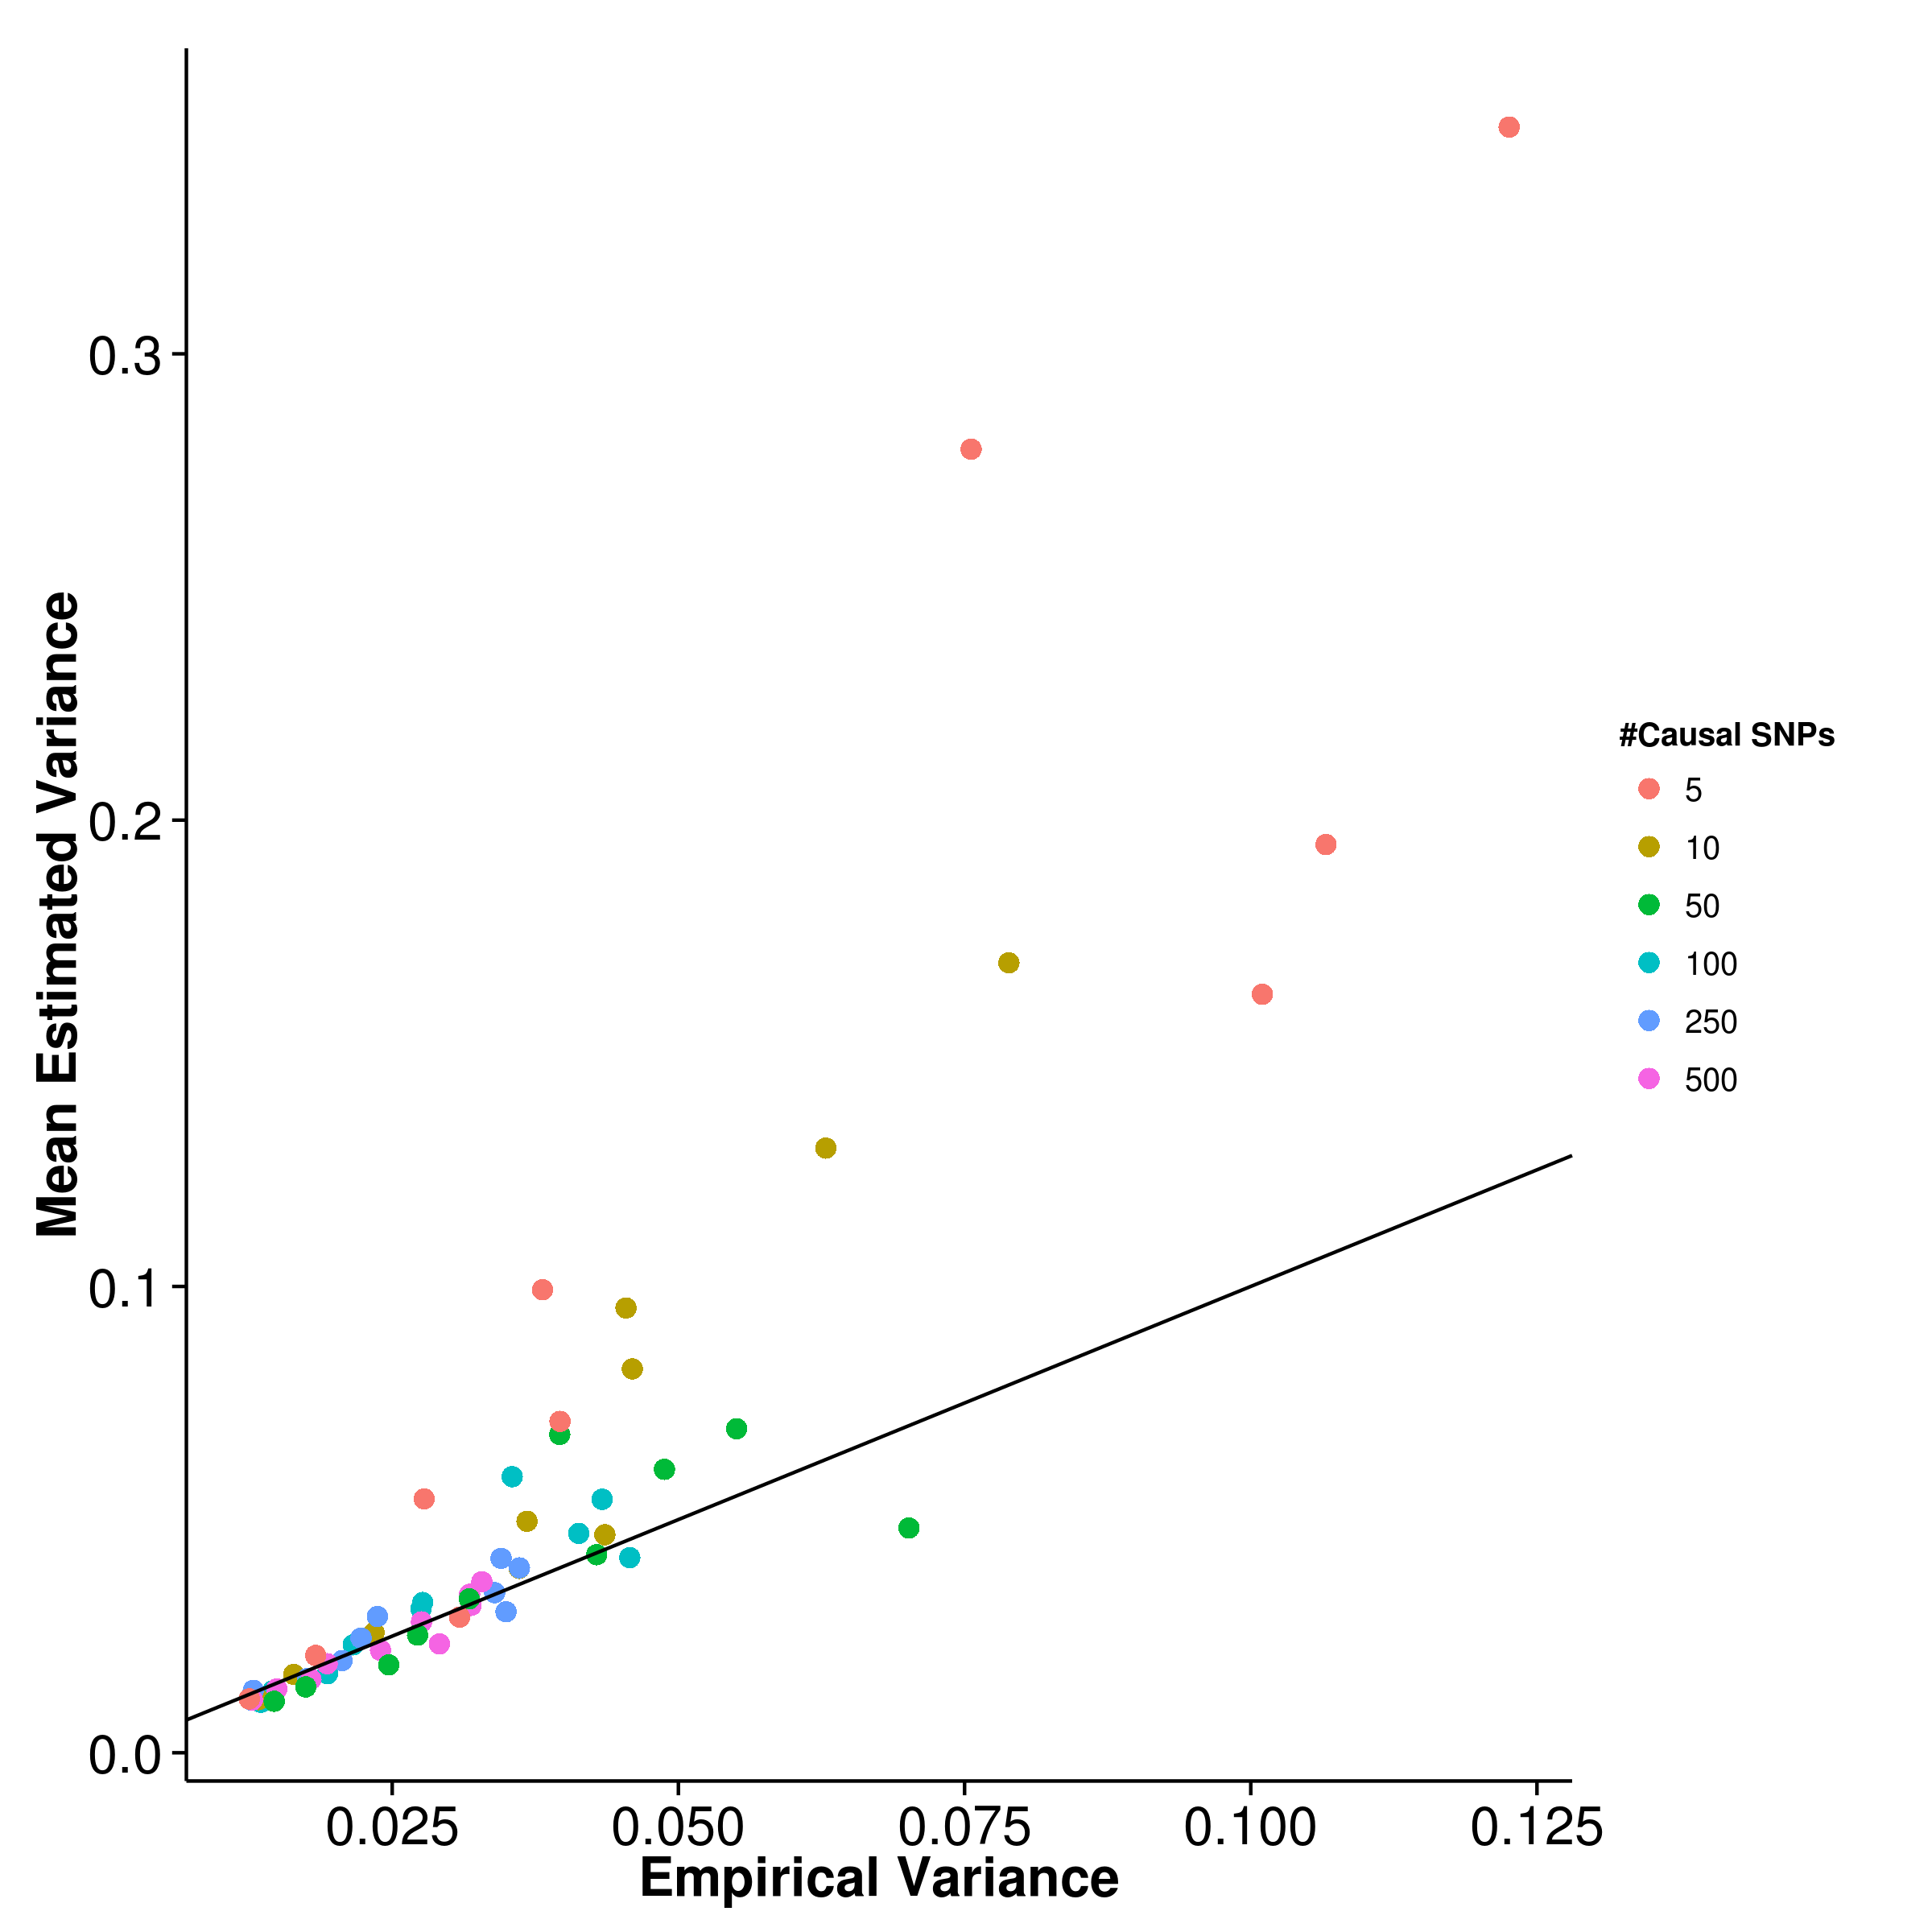
\includegraphics{figure/he_summary/random/ldscIn_Qt_Random_sdCom.png}}
				\label{fig:ldscInQtRandVarCom}
			}
			\caption[Quantitative Trait with Random Effect Size Simulation Result(Estimated Variance)]
			{Estimated variance of results from quantitative trait simulation with random effect size simulation when compared to the empirical variance.
				Similar to the simulation with equal effect size, the estimated variance seems to be affected by the number of causal \glspl{SNP}.
				} 
			\label{fig:QtRandVarCom}
		\end{figure}